
This section is focused on showing the main results of my investigation.
I start with discussing the dictionary of generated signals, 
then I move on to showing the results for motion-free simulations,
and I finalize with a discussion about the motion corrupted datasets.

% % % % % % % % % % % % % % % % % % % % % % % % % % % % % % % % % % % % % % % % % % % % % % % % % % % % % % % % % % % % % % % % % % % % % % % % % % % % % % % % % % % % % % % % % % % % % % % % % % % % % % % % % % % % % % % % % % % % % % % % % % % % % % % % % % % % % % % % % % % % % % % % % % % % % % % % % % % % % % % % % % % % % % % % 
\subsection{Dictionary Results}

Two sets of dictionaries were generated using the methods described in Section~\ref{method:dictionary}.
The acquisition sequence consisted of $N = 500$ repetition blocks, with both the repetition time and the echo time kept constant: $T_R = 15ms$ and $T_E = 7.5ms$.
The only sequence parameters that were varied from one acquisition to the next were the flip angles.
Figure~\ref{fig:FAsMaryia} shows the flip angles used for simulating the MRF dictionaries. 
% As the long term goal of my PhD project is to simulate the MRF-FISP sequence, I have chosen the shape of the flip angle distribution according to an MRF-FISP acquisition sequence which was used to acquire MRF data in a real experiment.

\begin{figure}[ht]
    \centering
    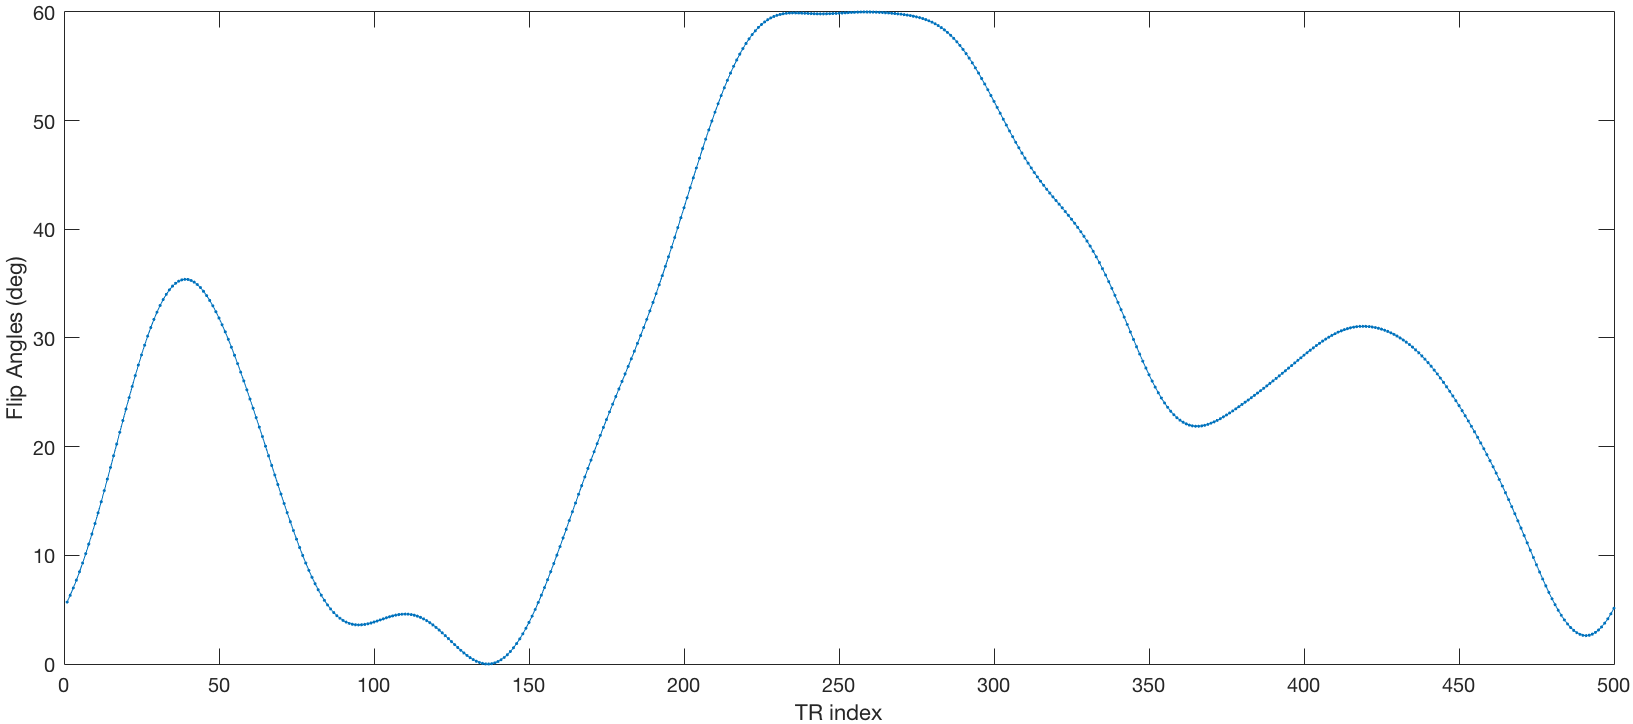
\includegraphics[width=1\textwidth]{images/mrf/FAsMaryia}
    \caption{The flip angles used for simulating the MRF dictionaries.
    The inversion pulse at the beginning of the RF pulse train is not shown here.}
    \label{fig:FAsMaryia}
\end{figure}

\hfill

The ranges of $T_1$ and $T_2$ values for this study were chosen to cover a wide range of typical relaxation times of the TO5 phantom.
Thus, $T_1$ values were chosen between $100ms$ and $2000ms$ with a $5ms$ increment, while
% $T_2$ values were chosen between $20ms$ and $200ms$ with a $5ms$ increment and between $350ms$ and $400ms$ with a $10ms$ increment.
% By applying both methods, two dictionaries, each consisting of $15,843$ entries with $500$ time points, were generated.
$T_2$ values were chosen between $20ms$ and $200ms$ with a $5ms$ increment and between $210ms$ and $400ms$ with a $10ms$ increment.
By applying both methods, two dictionaries, each consisting of $20,687$ entries with $500$ time points, were generated.
A set of representative dictionary entries are shown in Figure~\ref{fig:mrfDictionaries} with a),c) $T_1$ values ranging from $200ms$ to $800ms$ with $100ms$ increment and $T_2$ fixed to $20ms$; and b),d) $T_2$ values ranging from $20ms$ to $80ms$ with $10ms$ increment and $T_1$ fixed to $100ms$.
Next, I will describe some of the key features of the simulated signals.

\begin{figure}[ht]
    \centering
    \begin{subfigure}[b]{.75\textwidth}
        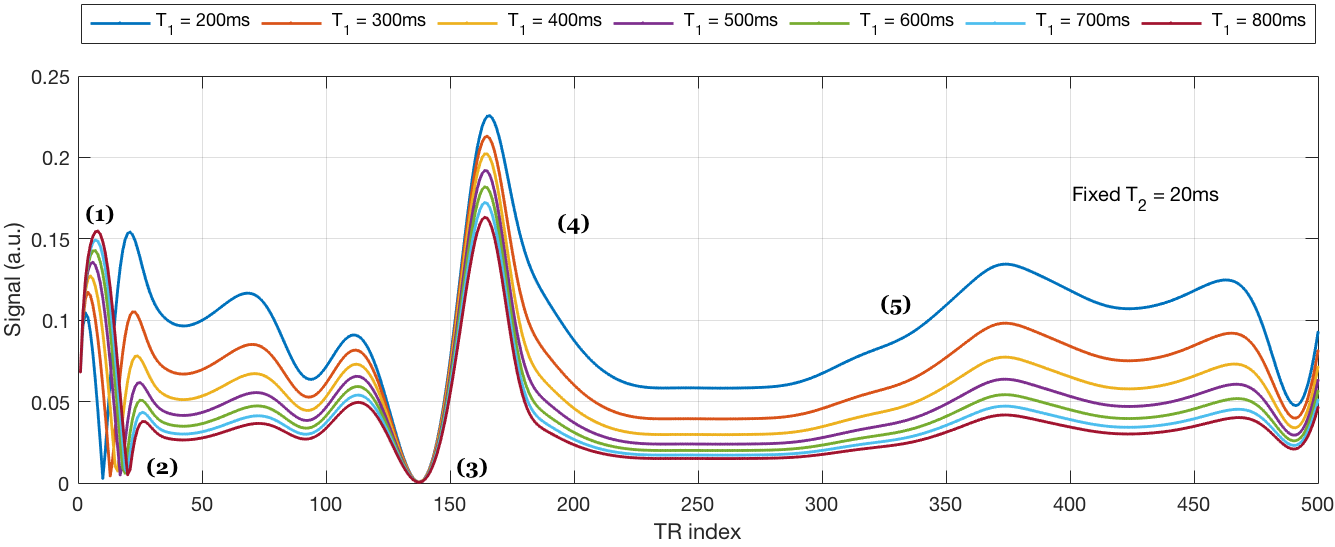
\includegraphics[width=\textwidth]{images/mrf/mrfDictionaryBSSFPaDesc}
        \caption{bSSFP fixed $T_2 = 20ms$}
    \end{subfigure}
    
    \begin{subfigure}[b]{.75\textwidth}
        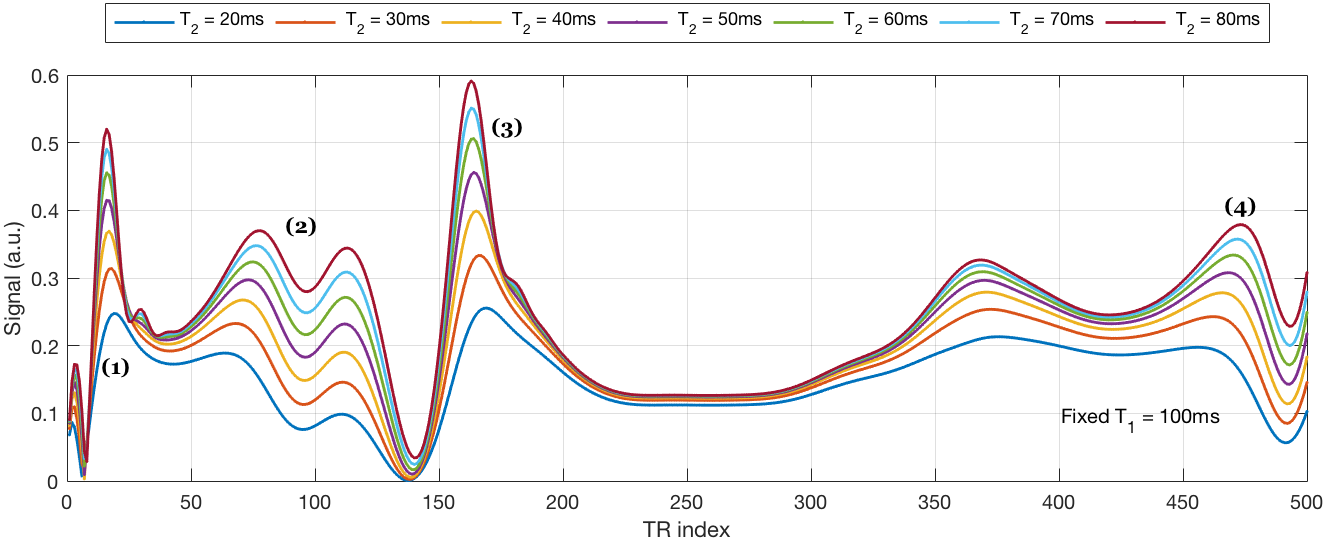
\includegraphics[width=\textwidth]{images/mrf/mrfDictionaryBSSFPbDesc}
        \caption{bSSFP fixed $T_1 = 100ms$}
    \end{subfigure}
    
    \begin{subfigure}[b]{.75\textwidth}
        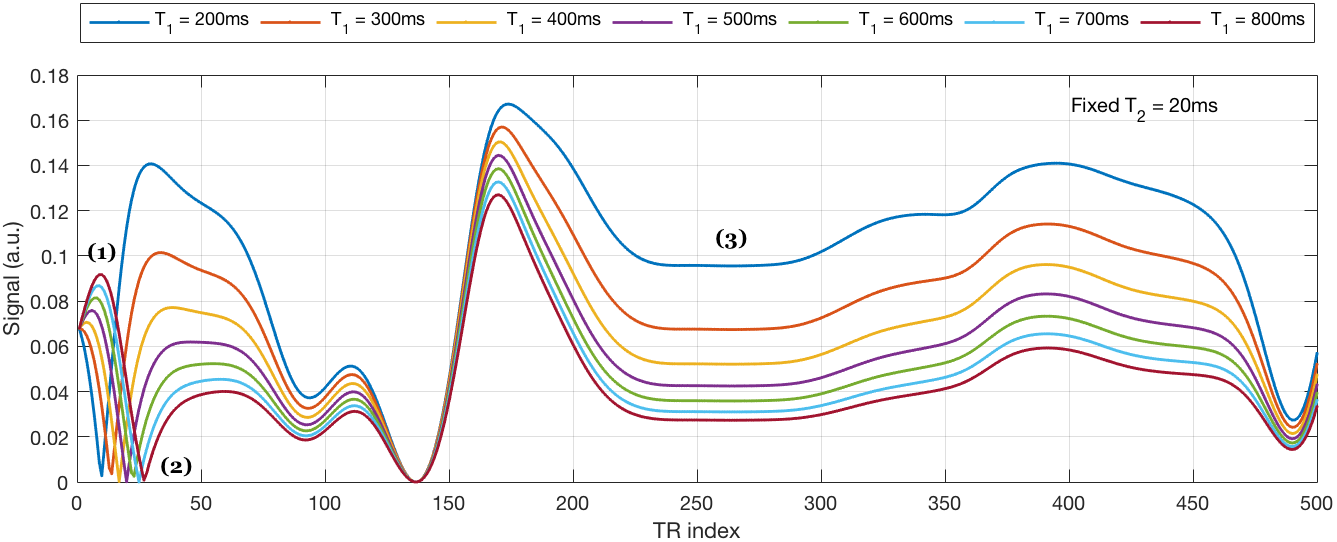
\includegraphics[width=\textwidth]{images/mrf/mrfDictionaryFISPaDesc}
        \caption{FISP fixed $T_2 = 20ms$}
    \end{subfigure}
    
    \begin{subfigure}[b]{.75\textwidth}
        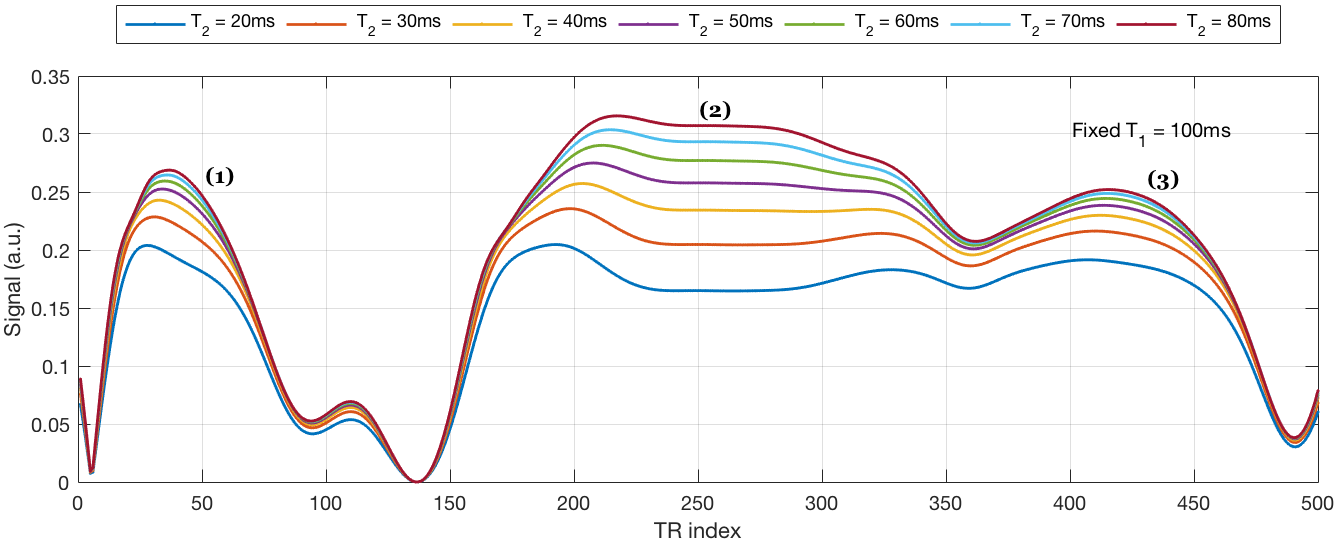
\includegraphics[width=\textwidth]{images/mrf/mrfDictionaryFISPbDesc}
        \caption{FISP fixed $T_1 = 100ms$}
    \end{subfigure}
    
    \caption{Example fingerprints for both the bSSFP and FISP dictionaries. In a) and c) we fix $T_2 = 20ms$ and we vary $T_1$ from $200ms$ to $800ms$ with $100ms$ increment, while in b) and d) we fix $T_1 = 100ms$ and we vary $T_2$ from $20ms$ to $80ms$ with $10ms$ increment.}
    \label{fig:mrfDictionaries}
\end{figure}

\hfill

% % % % Talk about the bSSFP dictionary
\textbf{bSSFP Dictionary.} 
Example fingerprints for the bSSFP dictionary are shown in the first two subplots of Figure~\ref{fig:mrfDictionaries}.
In \textbf{a)} the transverse relaxation time is kept fixed. 
The difference in shape between the fingerprints is due solely to their $T_1$ relaxation times.
The $180^o$ inversion pulse makes the fingerprints more easily distinguishable from the beginning:
a slower longitudinal relaxation time ($T_1 = 800ms$) means that at the beginning of the sequence there is more magnetisation to be flipped in the transverse plane, while a faster longitudinal relaxation time ($T_1 = 200ms$) will cause the opposite effect (1).
After a while, as the shorter $T_1$s help the magnetisation vector reach equilibrium faster, these fingerprints will have a stronger contribution to the signal and the signal trends will switch (2).

\hfill

By the $140^{th}$ pulse the flip angle values get closer to $0$. 
As a consequence of that, we can see a lack of signal at the same TR index (3).
This also allows the magnetisation vector to relax and give more signal as the flip angles increase in magnitude (4).
Moreover, as the flip angles are continuously varied, the signal is not allowed to reach steady state, but is kept in its transient phase which also allows for better discrimination throughout the sequence (5).

\hfill

In \textbf{b)} the longitudinal relaxation time is kept fixed and the difference in shapes between these fingerprints is due to their $T_2$ relaxation times.
Now, these signals are better discriminated from each other as the flip angles vary (see (1)-(4)): this keeps the signal in the transient phase and does not allow it to reach steady state.
Moreover, slower transverse relaxation times ($T_2 = 80ms$) will allow for more signal, while faster transverse relaxation times ($T_2 = 20ms$) will have the opposite effect.
This trend is seen throughout the entire acquisition.

\hfill

% % % % Talk about the FISP dictionary
\textbf{FISP Dictionary.} 
Example fingerprints for the FISP dictionary are shown in the last two subplots of Figure~\ref{fig:mrfDictionaries}.
The first feature to be noticed is that these signals have an overall lower magnitude than the ones for bSSFP.
This is a known consequence of using dephasing gradients and is explained in Appendix \ref{MRIFISP}.

\hfill

In \textbf{c)} the transverse relaxation time is kept fixed. 
Same as before, the difference in shapes between the fingerprints is due to their $T_1$ relaxation times and the $180^o$ inversion pulse makes the fingerprints more easily distinguishable at the beginning (1).
After some time, as the magnetisation vector relaxes towards thermal equilibrium and becomes positive, the signal trends will flip (2).
From this moment on, throughout the entire sequence, the faster longitudinal relaxation time ($T_1 = 200ms$) will give the higher signal, while the slowest longitudinal relaxation time ($T_1 = 800ms$) will give the lowest signal (3), as expected.

\hfill

In \textbf{d)} the longitudinal relaxation time is kept fixed and, as before, the difference in shapes between the fingerprints is due to their $T_2$ relaxation times.
Now, throughout the sequence, the higher $T_2$ values will give higher signal than the lowest $T_2$ values.
This is because the magnetisation vector will relax slower for the higher values and faster for the lower values by the readout time.
Moreover, these signals are better discriminated from each other as the flip angles get bigger (see (1)-(3), where $FA \geq 30^o$).
This is expected as very small flip angles will cause less magnetisation to be tipped in the transverse plane.

\hfill

For the remainder of this work we will only use the bSSFP dictionary.
This is because the image space simulations were done using a balanced steady state sequence.
The FISP sequence requires more computational power and it is in our future work.
Next, we will discuss the motion free and motion corrupted results.

% % % % % % % % % % % % % % % % % % % % % % % % % % % % % % % % % % % % % % % % % % % % % % % % % % % % % % % % % % % % % % % % % % % % % % % % % % % % % % % % % % % % % % % % % % % % % % % % % % % % % % % % % % % % % % % % % % % % % % % % % % % % % % % % % % % % % % % % % % % % % % % % % % % % % % % % % % % % % % % % % % % % % % % % 
\clearpage
\subsection{Image Space Simulations Results}

Ten different quantitative maps were generated using the methods described in Sections \ref{method:imagespace} and \ref{method:matching}, corresponding to one motion free dataset and 9 motion corrupted datasets.
The acquisition scheme was a balanced steady state free precession sequence with $N = 500$ repetition blocks, and constant $T_R = 15ms$ and $T_E = 7.5ms$.
Similar to the dictionary generation part, the only sequence parameters that were varied from one acquisition to the next were the flip angles (Figure~\ref{fig:FAsMaryia}).
Images from each acquisition block were reconstructed separately on an $128 \times 128$ matrix size using BART's \textsc{nufft} command line tool.
Then, a vector dot product was computed between the image space signals corresponding to every voxel position in the image dataset and the entire bSSFP dictionary and quantitative maps were created following the method described in Section \ref{method:matching}.

% T1/T2/Score maps no motion vs ground truth
\begin{figure}[ht]
    \centering
    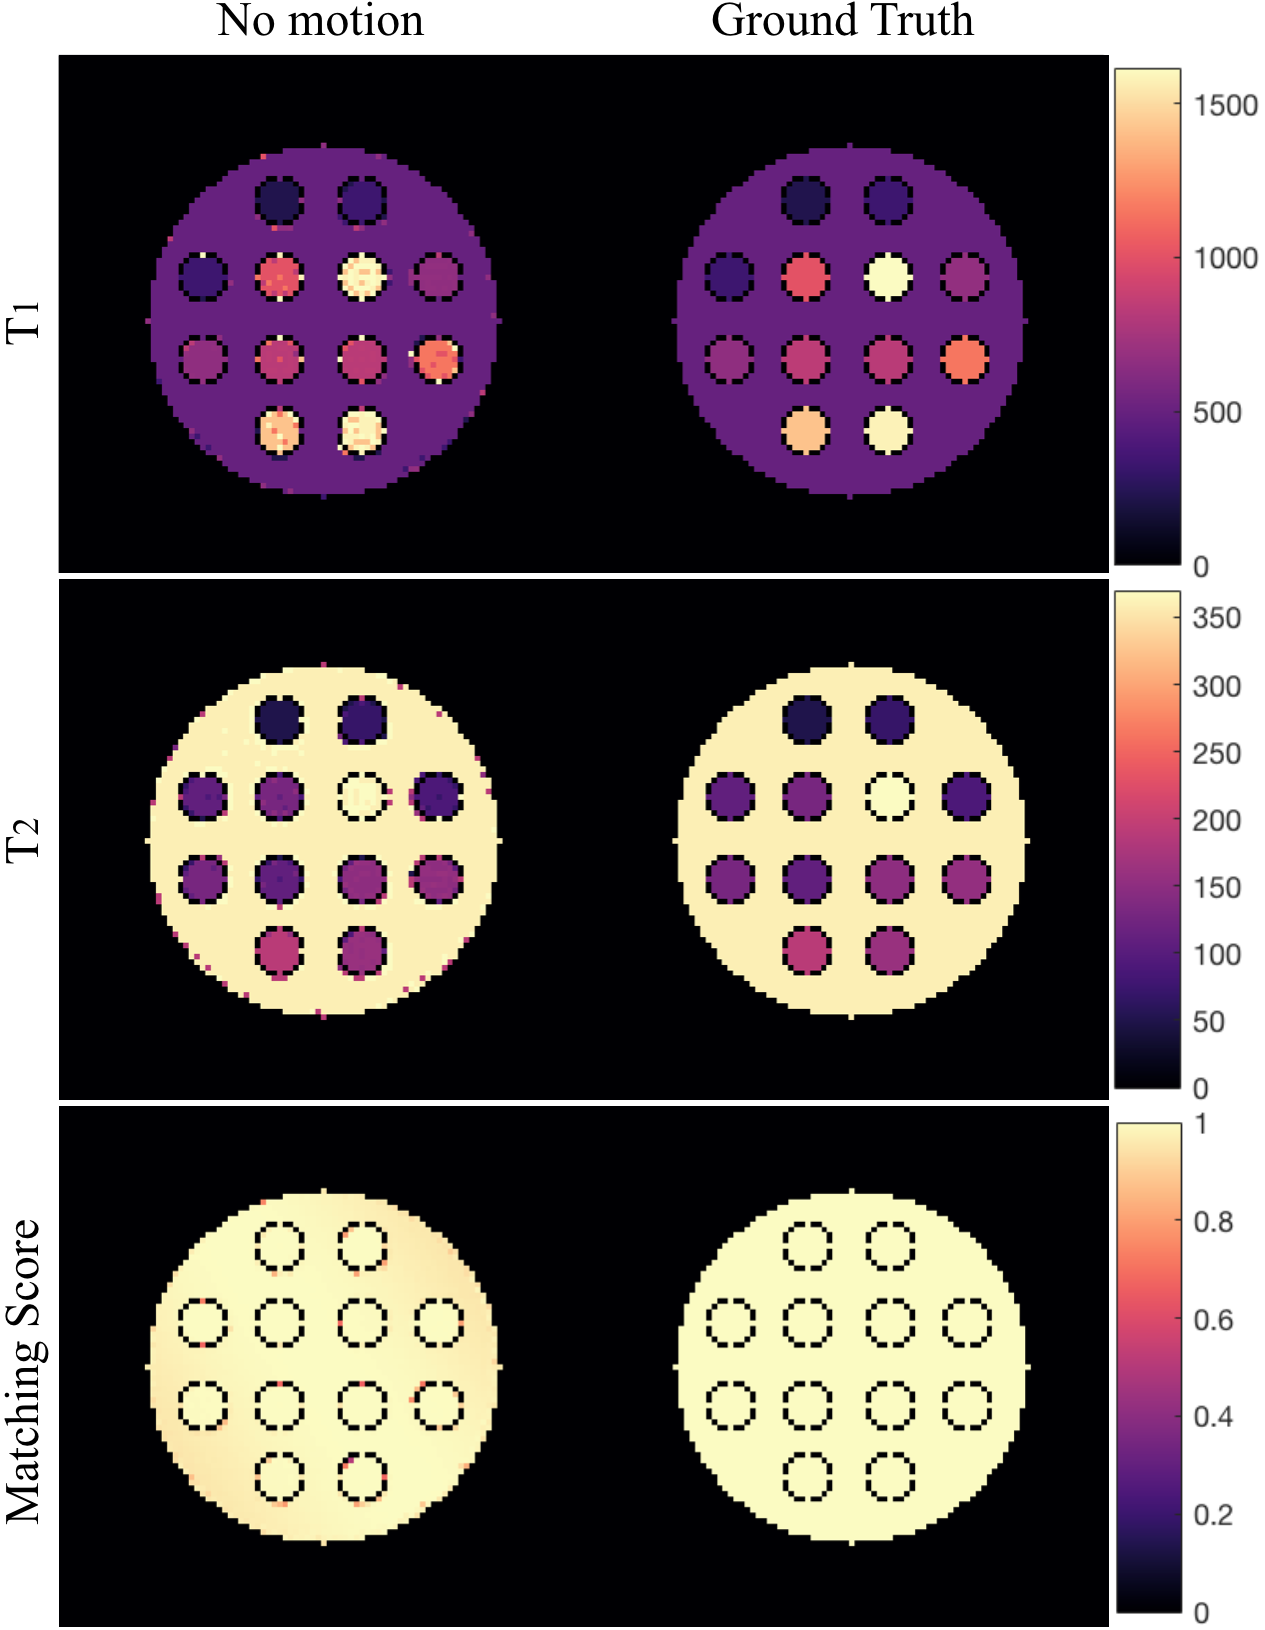
\includegraphics[width=0.6\textwidth]{images/mrf/T1T2ScoreNoMotion}
    \caption{$T_1$ and $T_2$ reconstructed maps together with the matching scores (column 1) and their corresponding ground truth values (column 2).}
    \label{fig:T1T2ScoreMapNoMotion}
\end{figure}

% % % % % % % % % % % % % % % % 
\subsubsection{Motion Free Results}
The first set of results corresponds to the motion free simulations.
These maps are shown in Figure~\ref{fig:T1T2ScoreMapNoMotion} where a mask was introduced to both eliminate the noise surrounding the object and to better distinguish the inner tubes from the bigger circle.
The results show that the reconstructed $T_1$ and $T_2$ maps are in good agreement with the ground truth values.
Moreover, the voxel-wise pattern matching scores are above 0.95 everywhere inside the reconstructed object.

\hfill

Figure~\ref{fig:nomotionExampleSignals} shows two examples of image space signals and their corresponding dictionary match.
Both matching scores are very high and the retrieved fingerprints correspond to the ground truth values. 

\begin{figure}[H]
    \centering
    \begin{subfigure}[b]{.7\textwidth}
        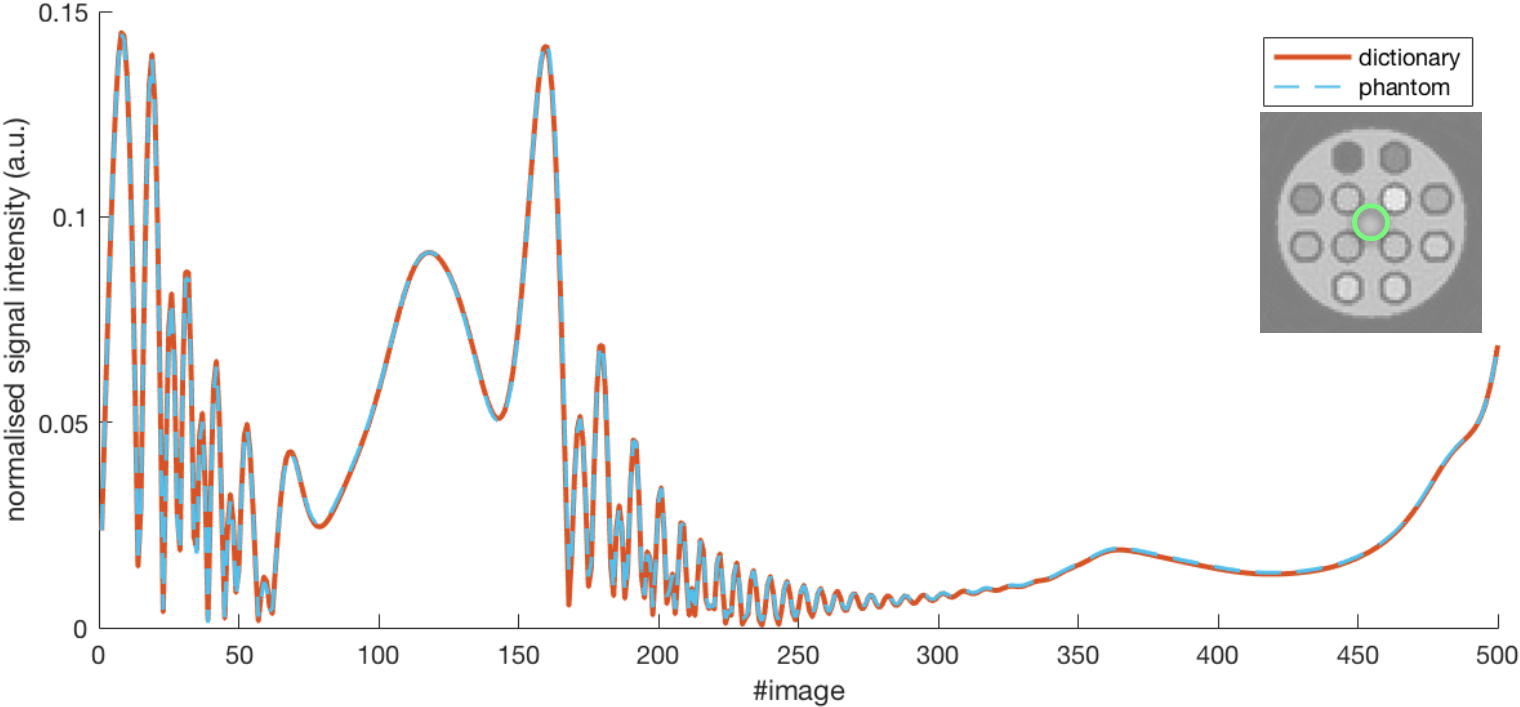
\includegraphics[width=\textwidth]{images/mrf/nomotionExampleSignalsa}
        \caption{The image space signal (blue dashed) matched to the fingerprint (red) corresponding to $T_1 = 500ms$ and $T_2 = 360ms$, with a matching score of 0.99.}
    \end{subfigure}
    
    \begin{subfigure}[b]{.7\textwidth}
        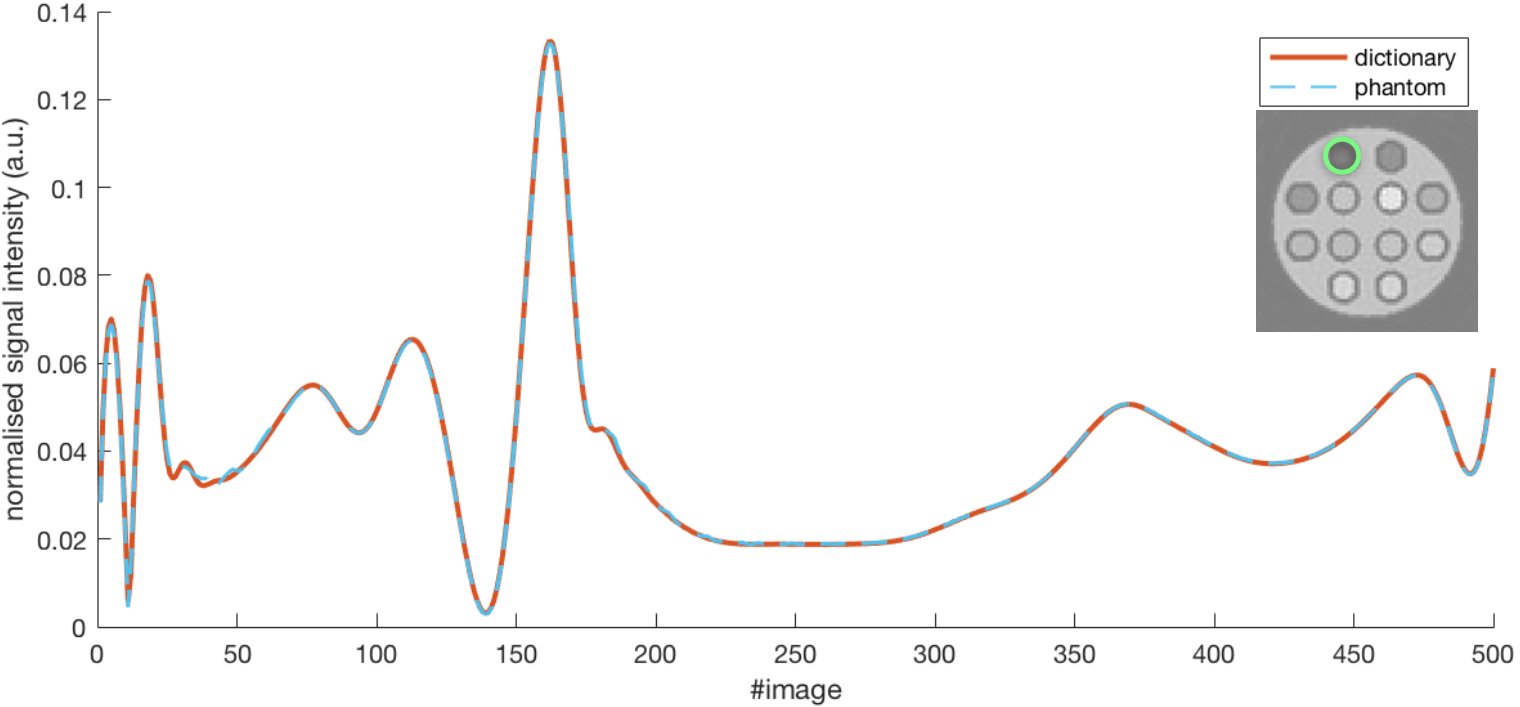
\includegraphics[width=\textwidth]{images/mrf/nomotionExampleSignalsb}
        \caption{The image space signal (blue dashed) matched to the fingerprint (red) corresponding to $T_1 = 225ms$ and $T_2 = 50ms$, with a matching score of 0.99}
    \end{subfigure}
    
    \caption{Example of image space signals matched to dictionary fingerprints for two different places within the phantom.
    Both results retrieve the correct ground truth values.}
    \label{fig:nomotionExampleSignals}
\end{figure}


% % % % % % % % % % % % % % % % 
\subsubsection{Motion Corrupted Results}

The second set of results corresponds to the motion corrupted simulations.
These maps are shown in Figure~\ref{fig:T1mapsmotion} and in Figure~\ref{fig:T2mapsmotion}, while the corresponding matching scores are in Appendix~\ref{appendixlabelMotion}.
Again, a mask was applied to eliminate the noise surrounding the object.

\hfill

The results show that, despite of the motion, the morphological structures of the phantom are well preserved in the $T_1$ and $T_2$ maps. 
However, the surrounding areas around each tube do not show the same sharpness as before.
Qualitatively, both $T_1$ and $T_2$ maps seem to be most affected when motion happens at the beginning of the scan, while the least affected maps are those when motion happens in the middle of the scan.

\hfill

To quantify the deviations from the ground truth values, I performed a region of interest analysis.
This consisted of calculating the mean and standard deviation in the simulated $T_1$ and $T_2$ values obtained in each of the inner tubes of the digital phantom in the motion free and motion corrupted data set and comparing them to the ground truth values.
The difference in absolute value between the simulated results and the ground truth values are shown in Figure~\ref{fig:GTMinusSimuAbsoluteDifference} for both the $T_1$ maps and the $T_2$ maps.
The first important feature to observe in these results is that the region of interest positioned in the middle of the phantom is least affected by the motion.
This is to be expected for motion happening at any time point during the scan as the rotation's axis is going through this middle point and the translation is happening along a line which does not intersect any other structures.
Next, the figure also shows that reconstructed $T_1$ values are affected the most when the motion happens in the beginning or at the end of the scan, while the $T_2$ values are effected the most when the motion happens at the beginning of the scan.

\hfill

The most affected reconstructed values correspond to the $5^{th}$ tube for both $T_1$ and $T_2$ values, and for the $5^{th}$, the $11^{th}$ and the $12^{th}$ tubes for the $T_1$ values.
To understand why, I plot in Figure~\ref{fig:problematicfingerprints} the dictionary fingerprints corresponding to $T_1$ and $T_2$ values which are close to the problematic tubes.
Moreover, I highlight the areas where the motion is happening for the three different onsets.
When $T_2$ is fixed, the fingerprints are very close together, especially in the middle of the sequence.
This explains why the $T_1$ maps are mostly affected when motion happens in the beginning of the sequence as there is where the dictionary match carries more significance.
Also, the last 50 repetition blocks in the sequence show a `spread' in the signals, which can explain why the $T_1$ maps can also be affected when motion is happening at the end of the scan.
When $T_1$ is fixed, the fingerprints are close together in the middle and at the end, which explains why it is more important that the signals are matched correctly at the beginning of the scan and why the $T_2$ maps are mostly affected when that happens.

\begin{figure}[ht]
    \centering
    \begin{subfigure}[b]{.85\textwidth}
        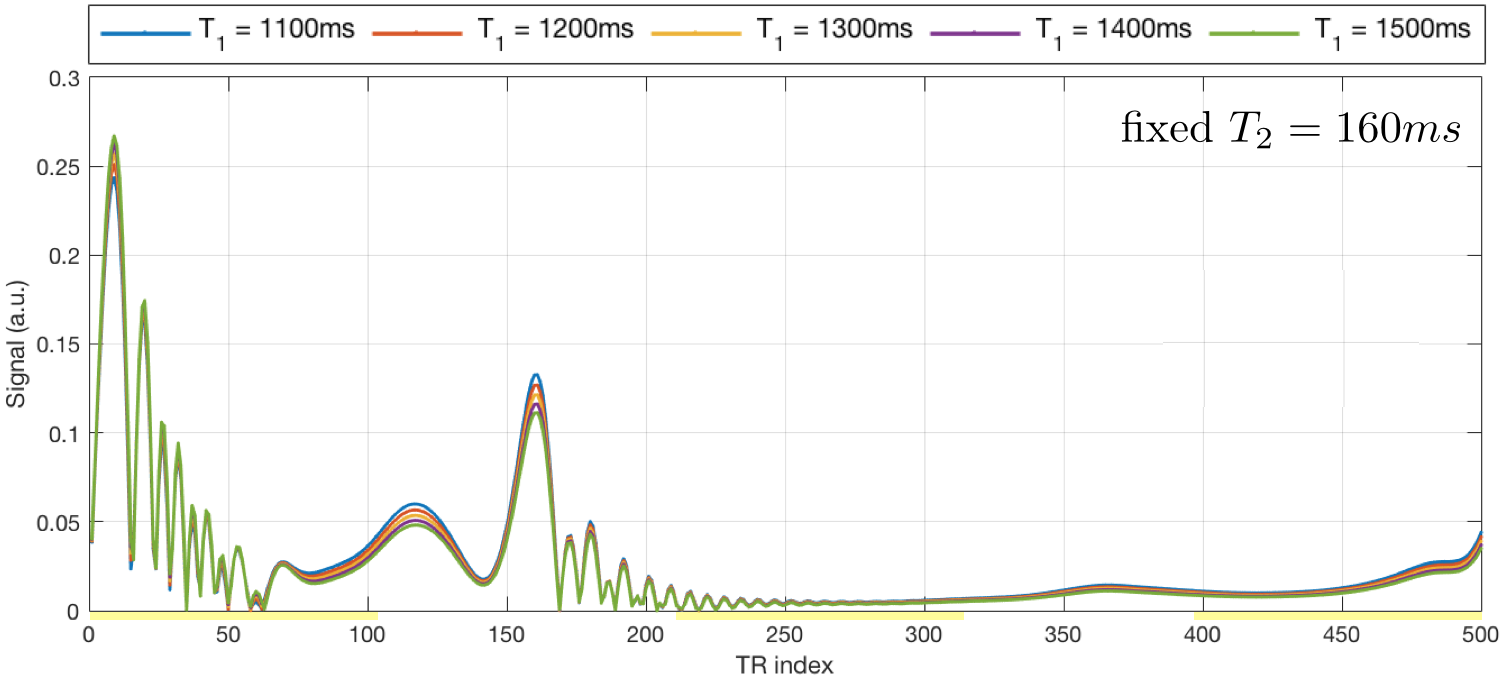
\includegraphics[width=\textwidth]{images/mrf/FixedT2VaryT1TubesMotion}
        \caption{Dictionary fingerprints corresponding to a range of $T_1$ values and a fixed $T_2$ value}
    \end{subfigure}
    
    \begin{subfigure}[b]{.85\textwidth}
        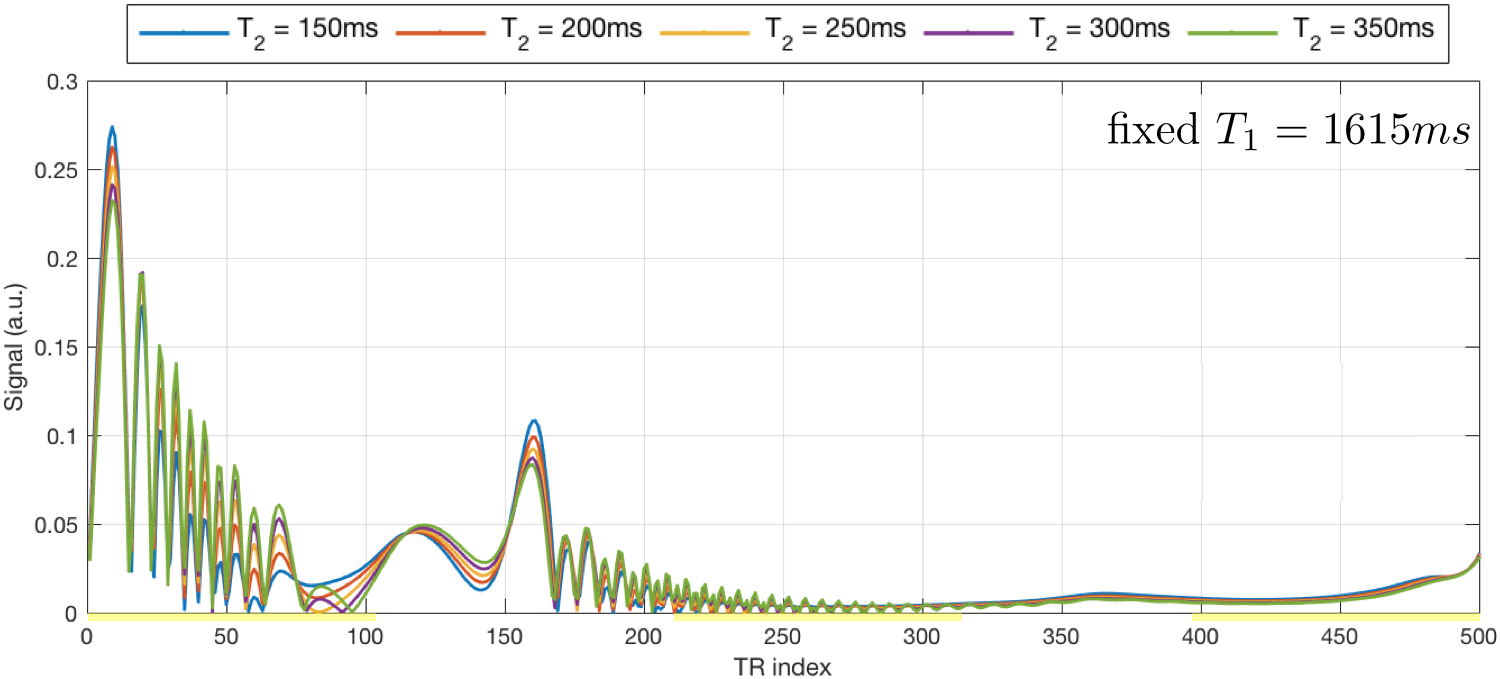
\includegraphics[width=\textwidth]{images/mrf/FixedT1VaryT2TubesMotion}
        \caption{Dictionary fingerprints corresponding to a range of $T_2$ values and a fixed $T_1$ value}
    \end{subfigure}
    
    \caption{Example fingerprints for $T_1$ and $T_2$ values corresponding to the most affected phantom tubes}
    \label{fig:problematicfingerprints}
\end{figure}

% ROI T1 and T2 average all simulated
\begin{figure}[ht]
    \centering
    \begin{subfigure}[b]{.9\textwidth}
        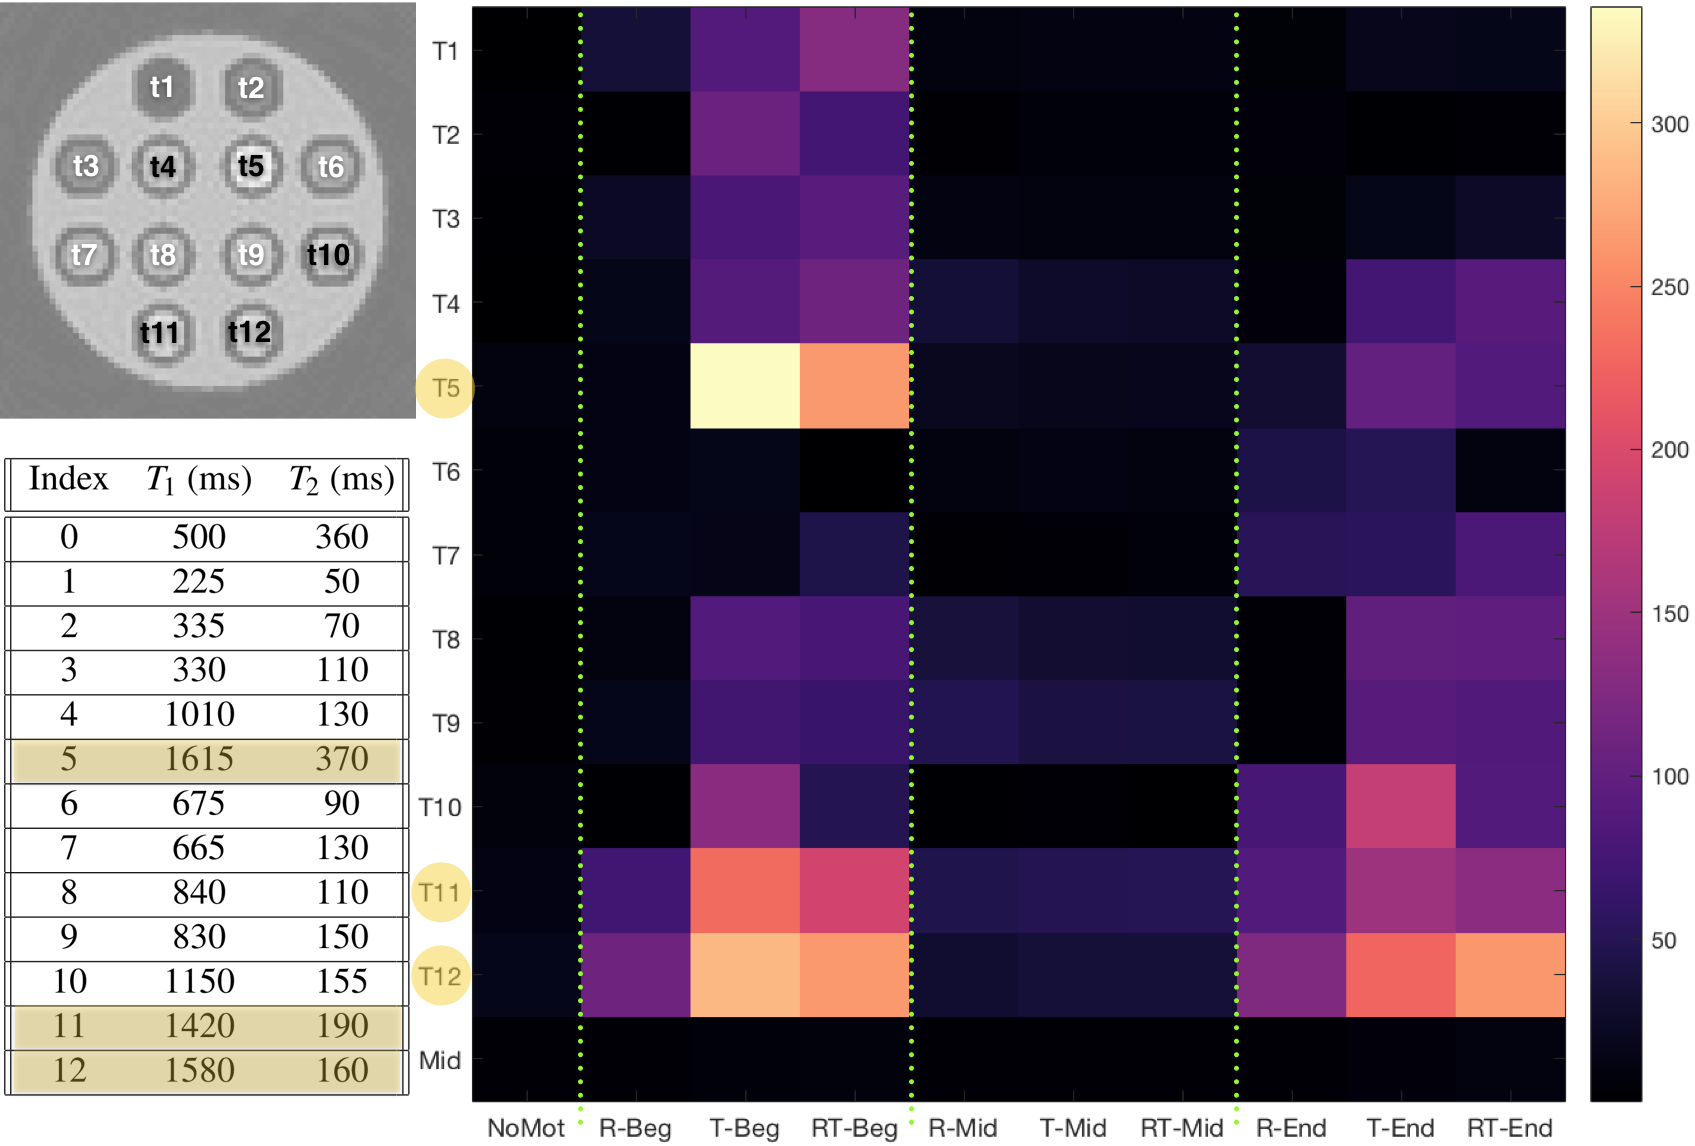
\includegraphics[width=\textwidth]{images/mrf/T1GTMinusT1SimuAbsoluteDifference}
        %\caption{$|T_1^{simulated} - T_1^{ground \, \, truth}|$}
        \label{fig:T1GTMinusT1SimuAbsoluteDifference}
    \end{subfigure}
    
    \begin{subfigure}[b]{.9\textwidth}
        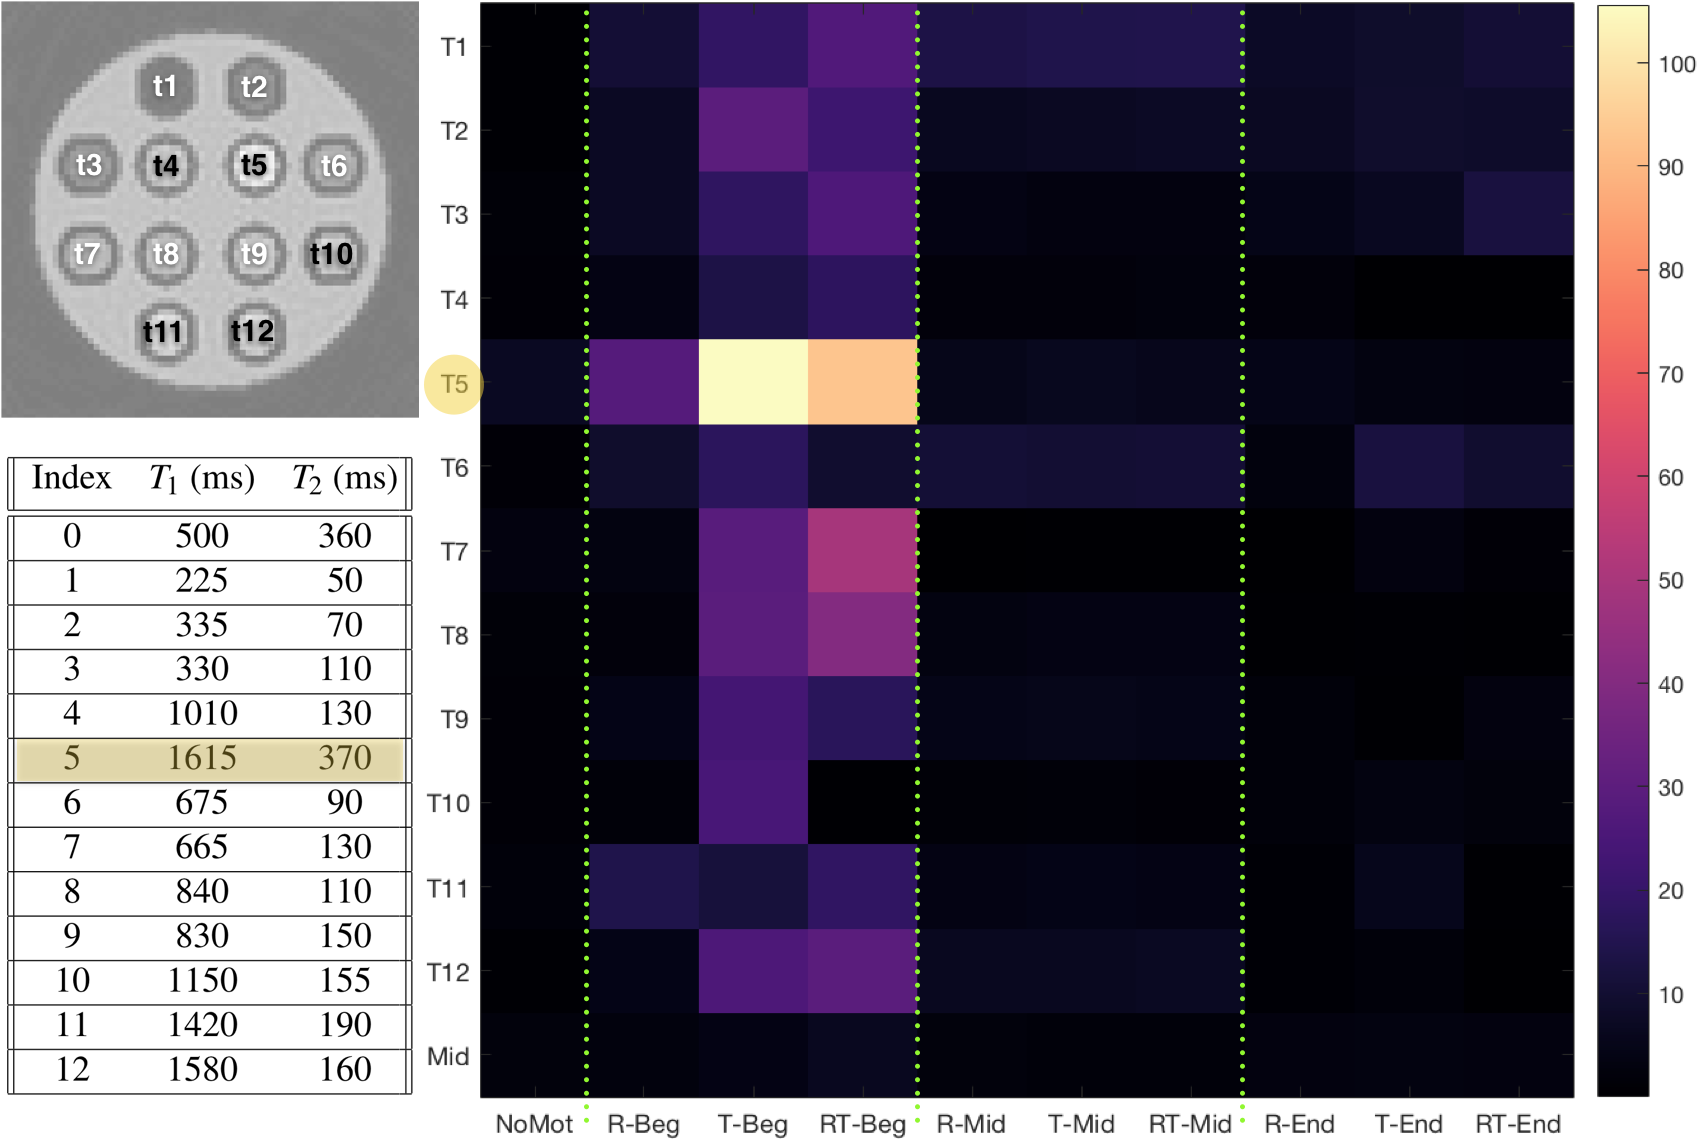
\includegraphics[width=\textwidth]{images/mrf/T2GTMinusT2SimuAbsoluteDifference}
        %\caption{$|T_2^{simulated} - T_2^{ground \, \, truth}|$}
        \label{fig:T2GTMinusT2SimuAbsoluteDifference}
    \end{subfigure}
    
    \caption{Region of interest analysis on the inner tubes (shown as $T_N$ in the plot) and middle of the phantom (shown as $Mid$ in the plot) for the simulated quantitative a) $T_1$  maps and b) $T_2$ maps.
    The plot shows the difference in absolute value between the simulated a) $T_1$ maps or b) $T_2$ maps and the ground truth values.
    Each line corresponds to a different part of the phantom, shown in the upper left corner of the figure, while different columns correspond to different motion types and onsets.
    The first column corresponds to the no motion case,
    while the rest correspond to all three types of motion with onset at:
    the beginning of the scan (first three columns),
    the middle of the scan (next three columns), and
    at the end of the scan (last three columns).
    The ground truth values are found in the table, where the tubes with the highest difference in absolute values for all motion types were highlighted.}
    \label{fig:GTMinusSimuAbsoluteDifference}
\end{figure}

% For this, I chose 4 of the inner tubes, corresponding to the $1^{st}$, $3^{rd}$, $5^{th}$ and $12^{th}$ tube, and also an ROI positioned in the middle of the phantom.
% The results for ground truth, motion free and different onsets of \textit{motion 1} are shown in Figure~\ref{fig:motion1ROI}.
% The other two types of motion are found in Appendix~\ref{appendixlabelMotion}, in Figure~\ref{fig:appendixmotion2ROI} and Figure~\ref{fig:appendixmotion3ROI}.

% % ROI analysis motion 1
% \begin{figure}[ht]
%     \makebox[\textwidth][c]{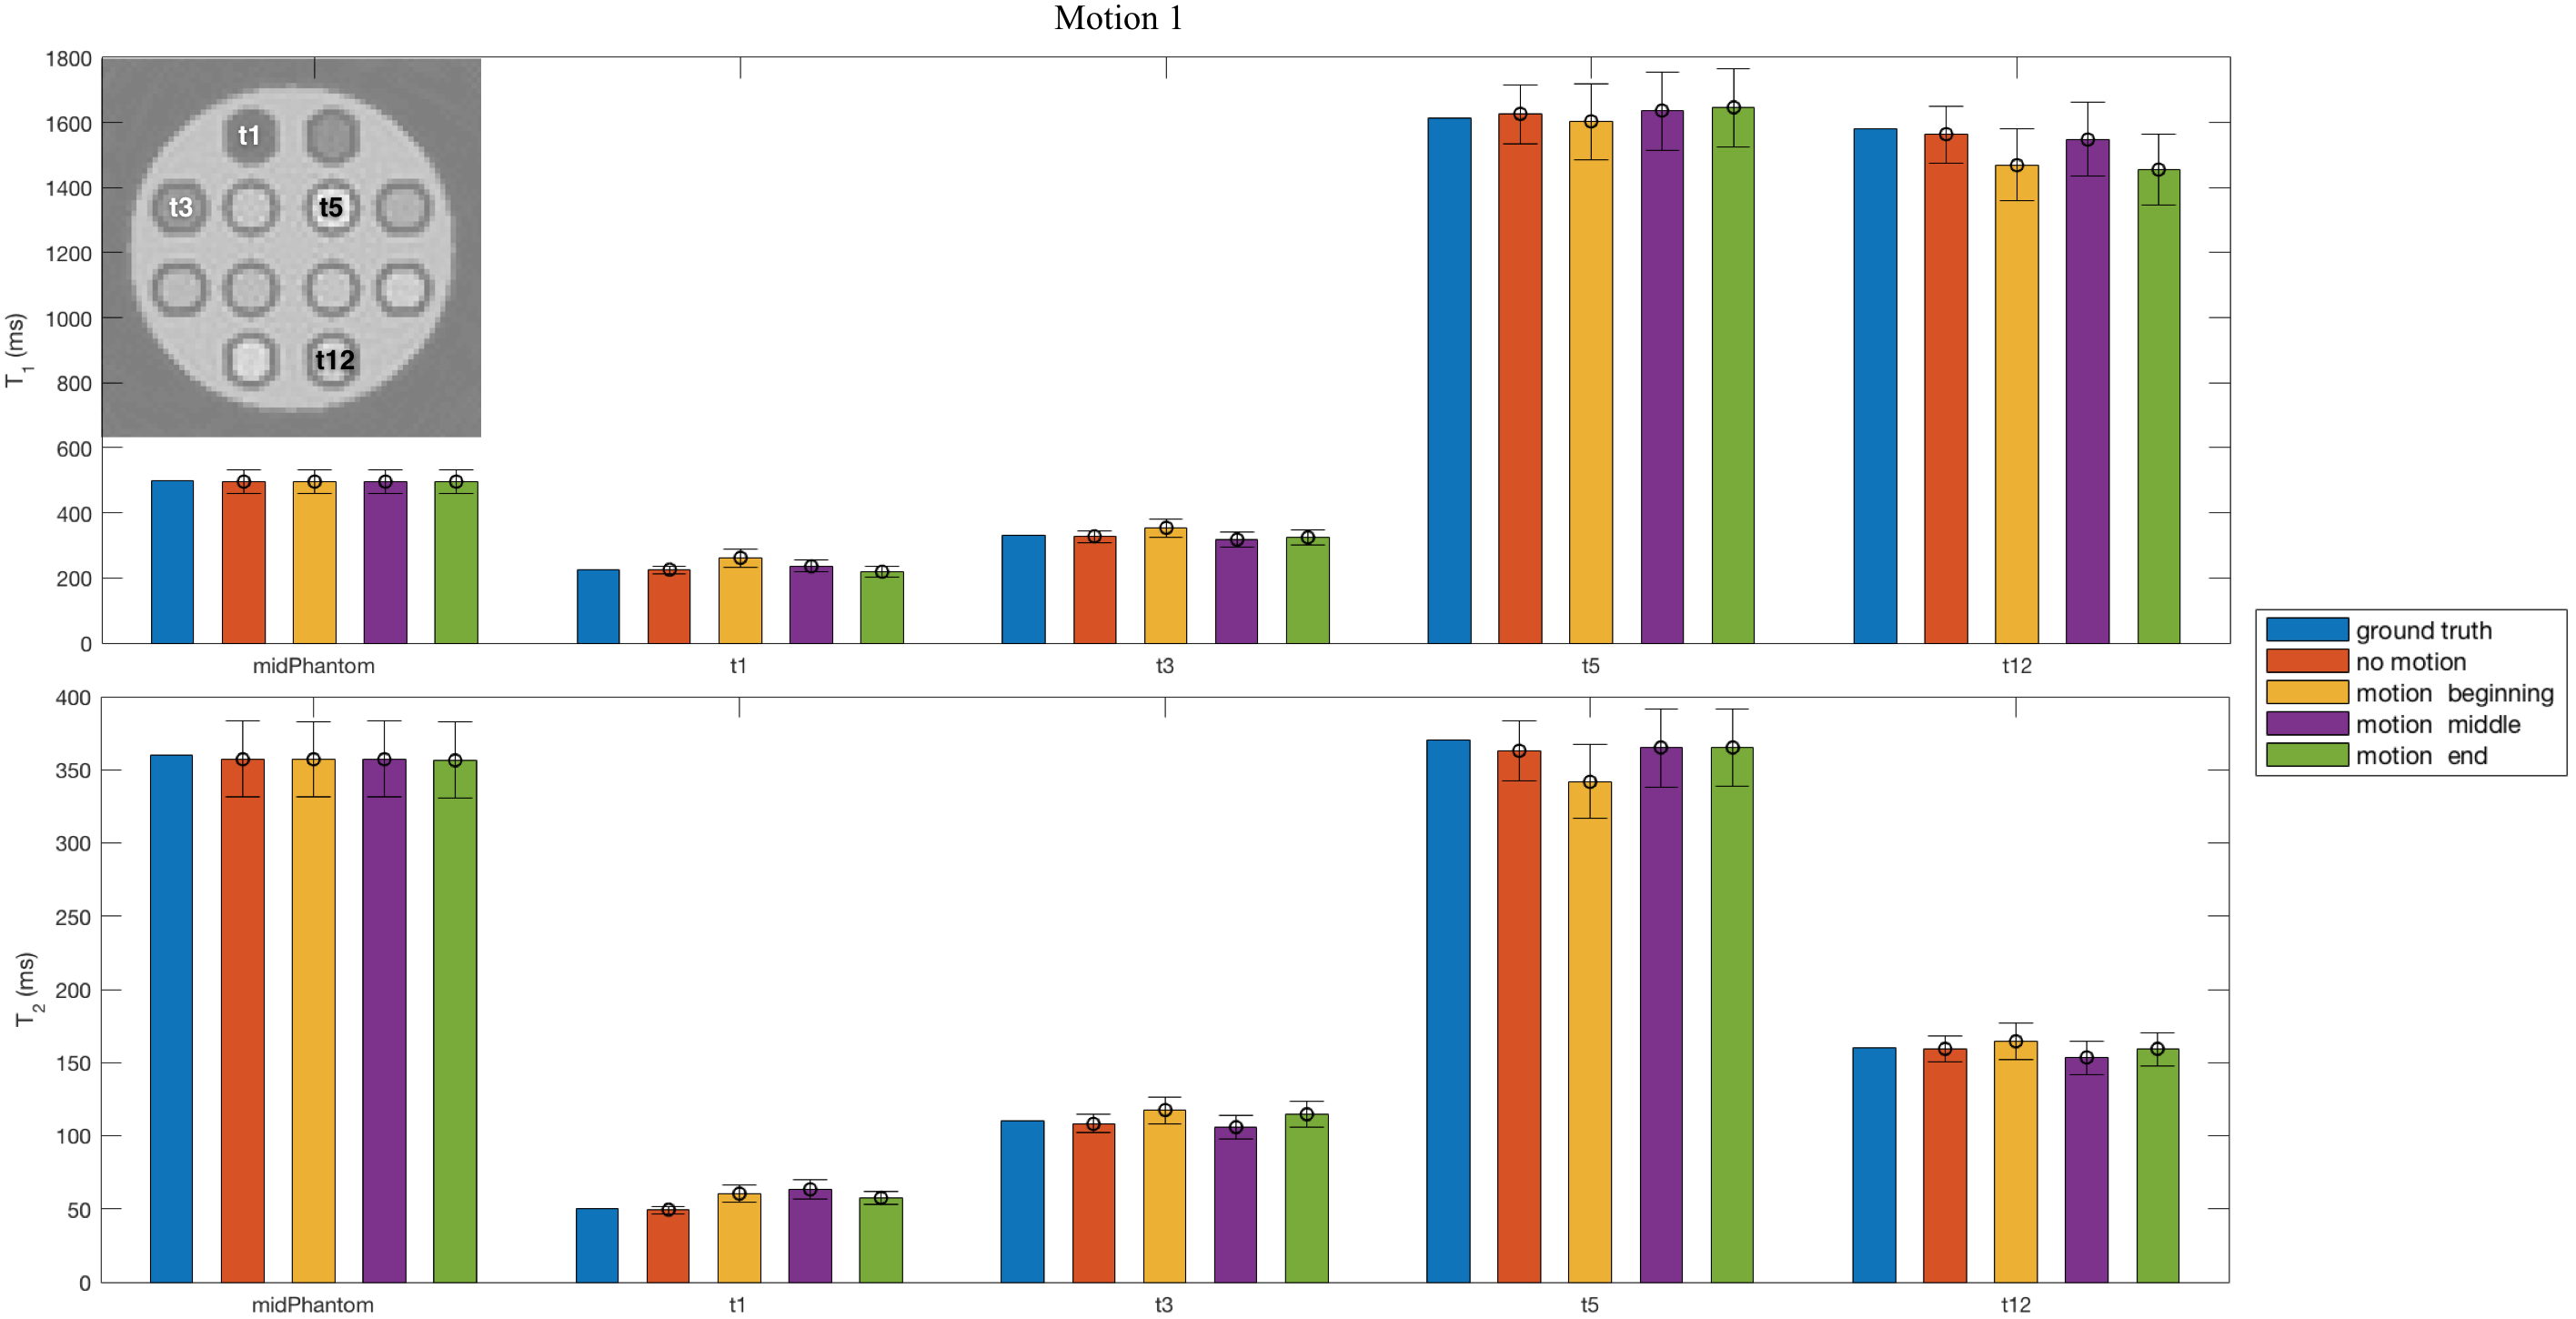
\includegraphics[width=1.3\textwidth]{images/mrf/motion1ROI}}
%     \caption{Region of interest analysis on \textit{motion 1} for different motion onsets}
%     \label{fig:motion1ROI}
% \end{figure}

\hfill

% The first important feature to observe in these results is that the region of interest positioned in the middle of the phantom is least affected by the motion.
% This is to be expected for motion happening at any time point during the scan as the rotation's axis is going through this middle point and the translation is happening along a line which does not intersect any other materials.

% % % Put images here:
% T1 maps motion
\begin{figure}[ht]
    \centering
    \begin{subfigure}[b]{.65\textwidth}
        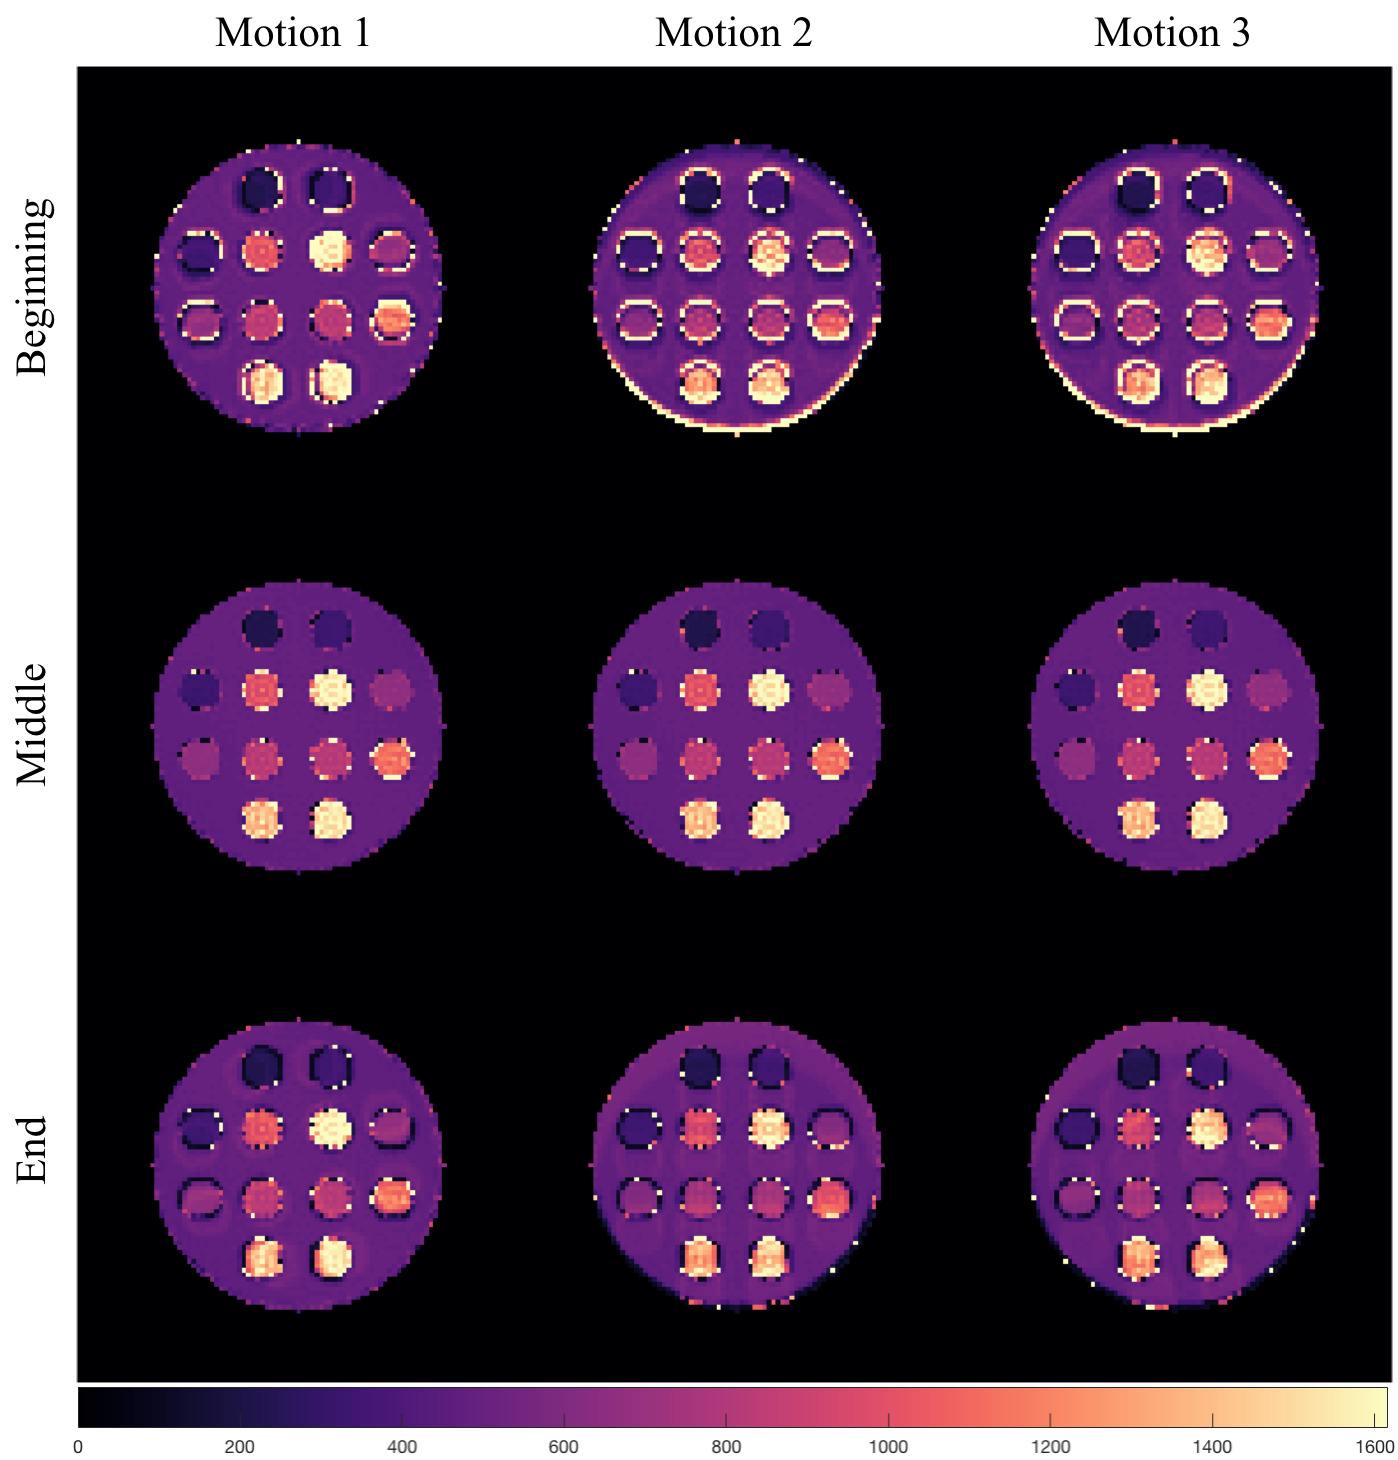
\includegraphics[width=\textwidth]{images/mrf/T1mapsmotion}
        \caption{Motion corrupted $T_1$ maps}
    \end{subfigure}
    
    \begin{subfigure}[b]{.65\textwidth}
        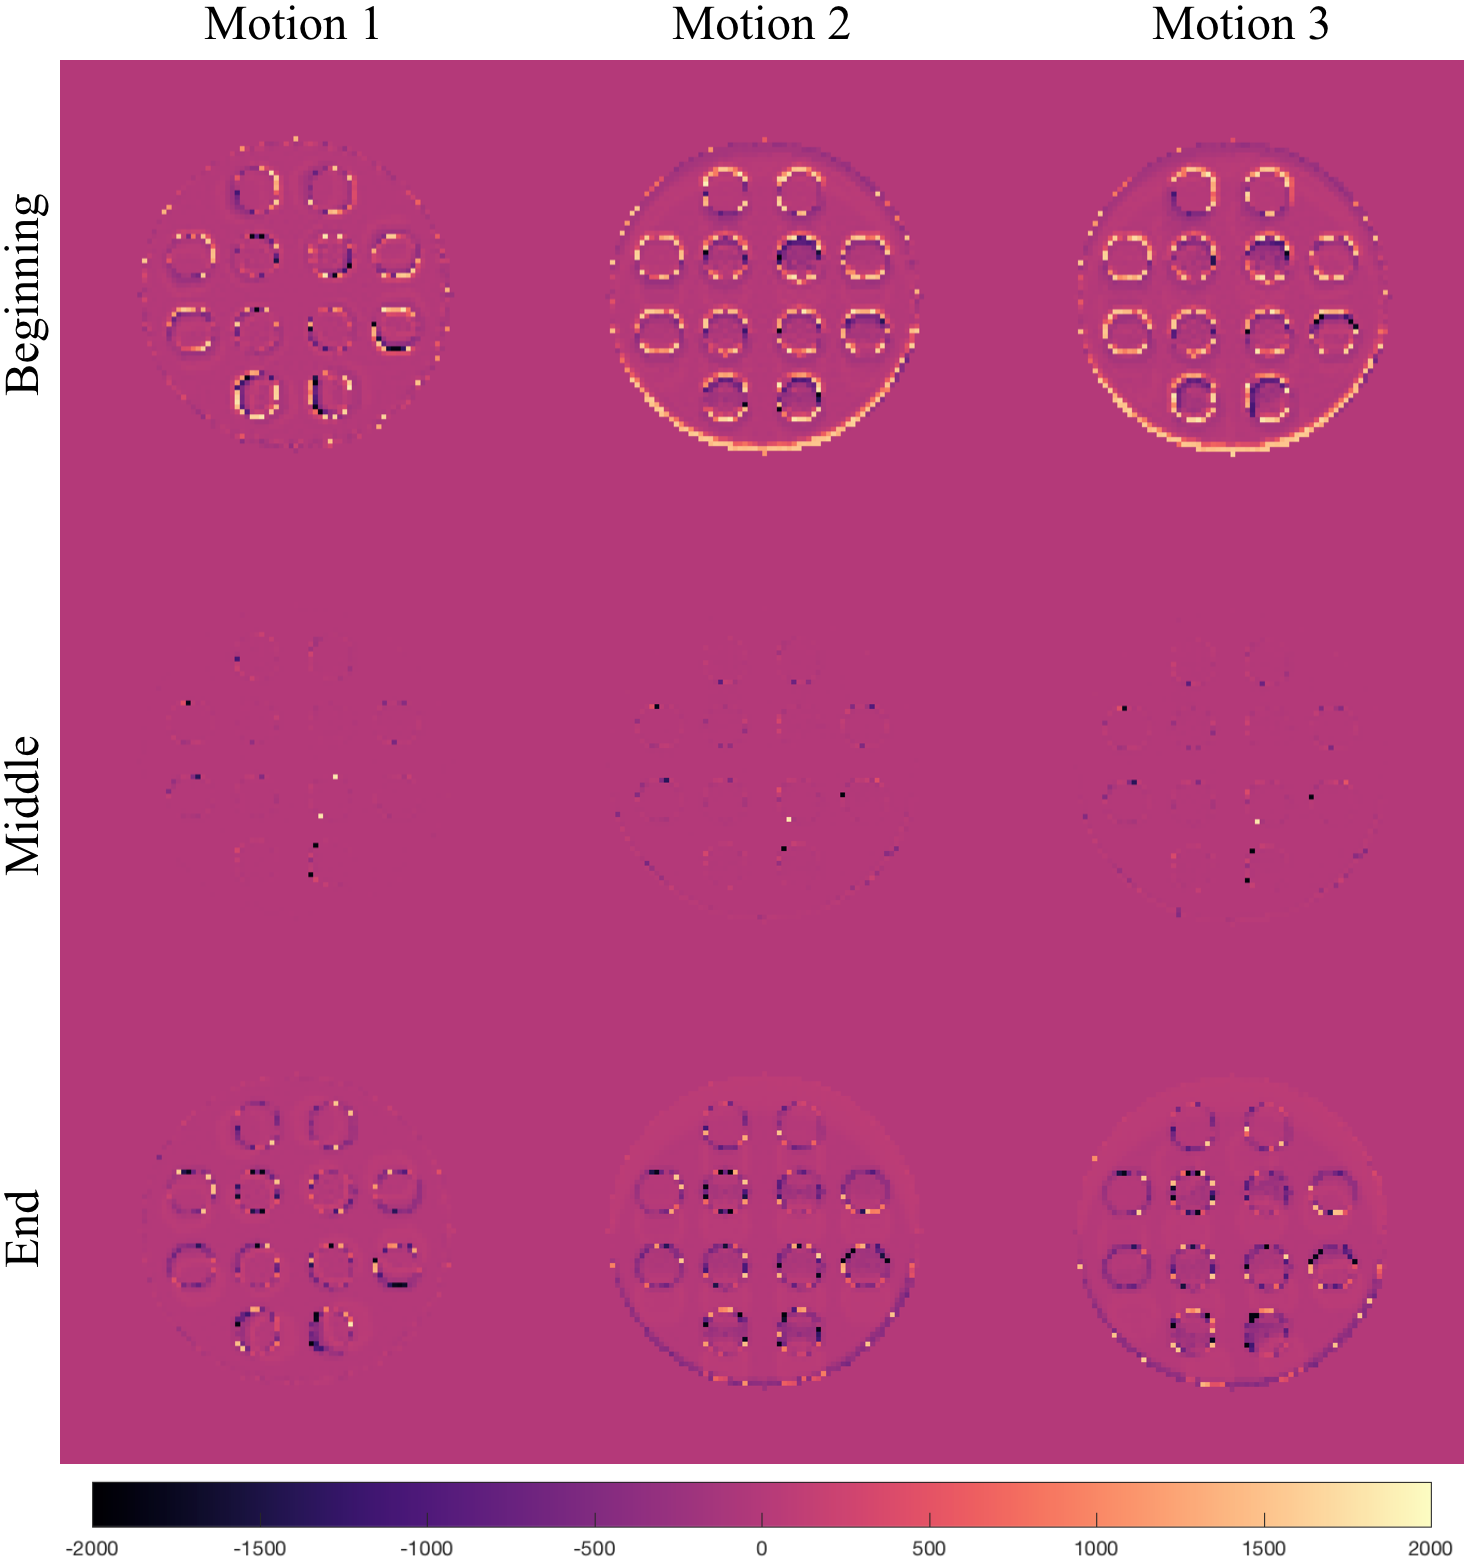
\includegraphics[width=\textwidth]{images/mrf/T1SimuMinusT1Real}
        \caption{Difference between $T_1^{motion \, \, corrupted}$ and $T_1^{motion \, \, free}$}
    \end{subfigure}
    
    \caption{Motion corrupted $T_1$ quantitative maps for all 9 types of motion traces. First column corresponds to the \textit{motion 1} trace (continuous rotation about the z-axis), the second column corresponds to the \textit{motion 2} trace (continuous translation along the y-axis) and the third column corresponds to the \textit{motion 3} trace (continuous rotation about the z-axis and continuous translation along the y-axis). Different lines correspond to a different onset of motion.}
    \label{fig:T1mapsmotion}
\end{figure}
% \begin{figure}[ht]
%     \centering
%     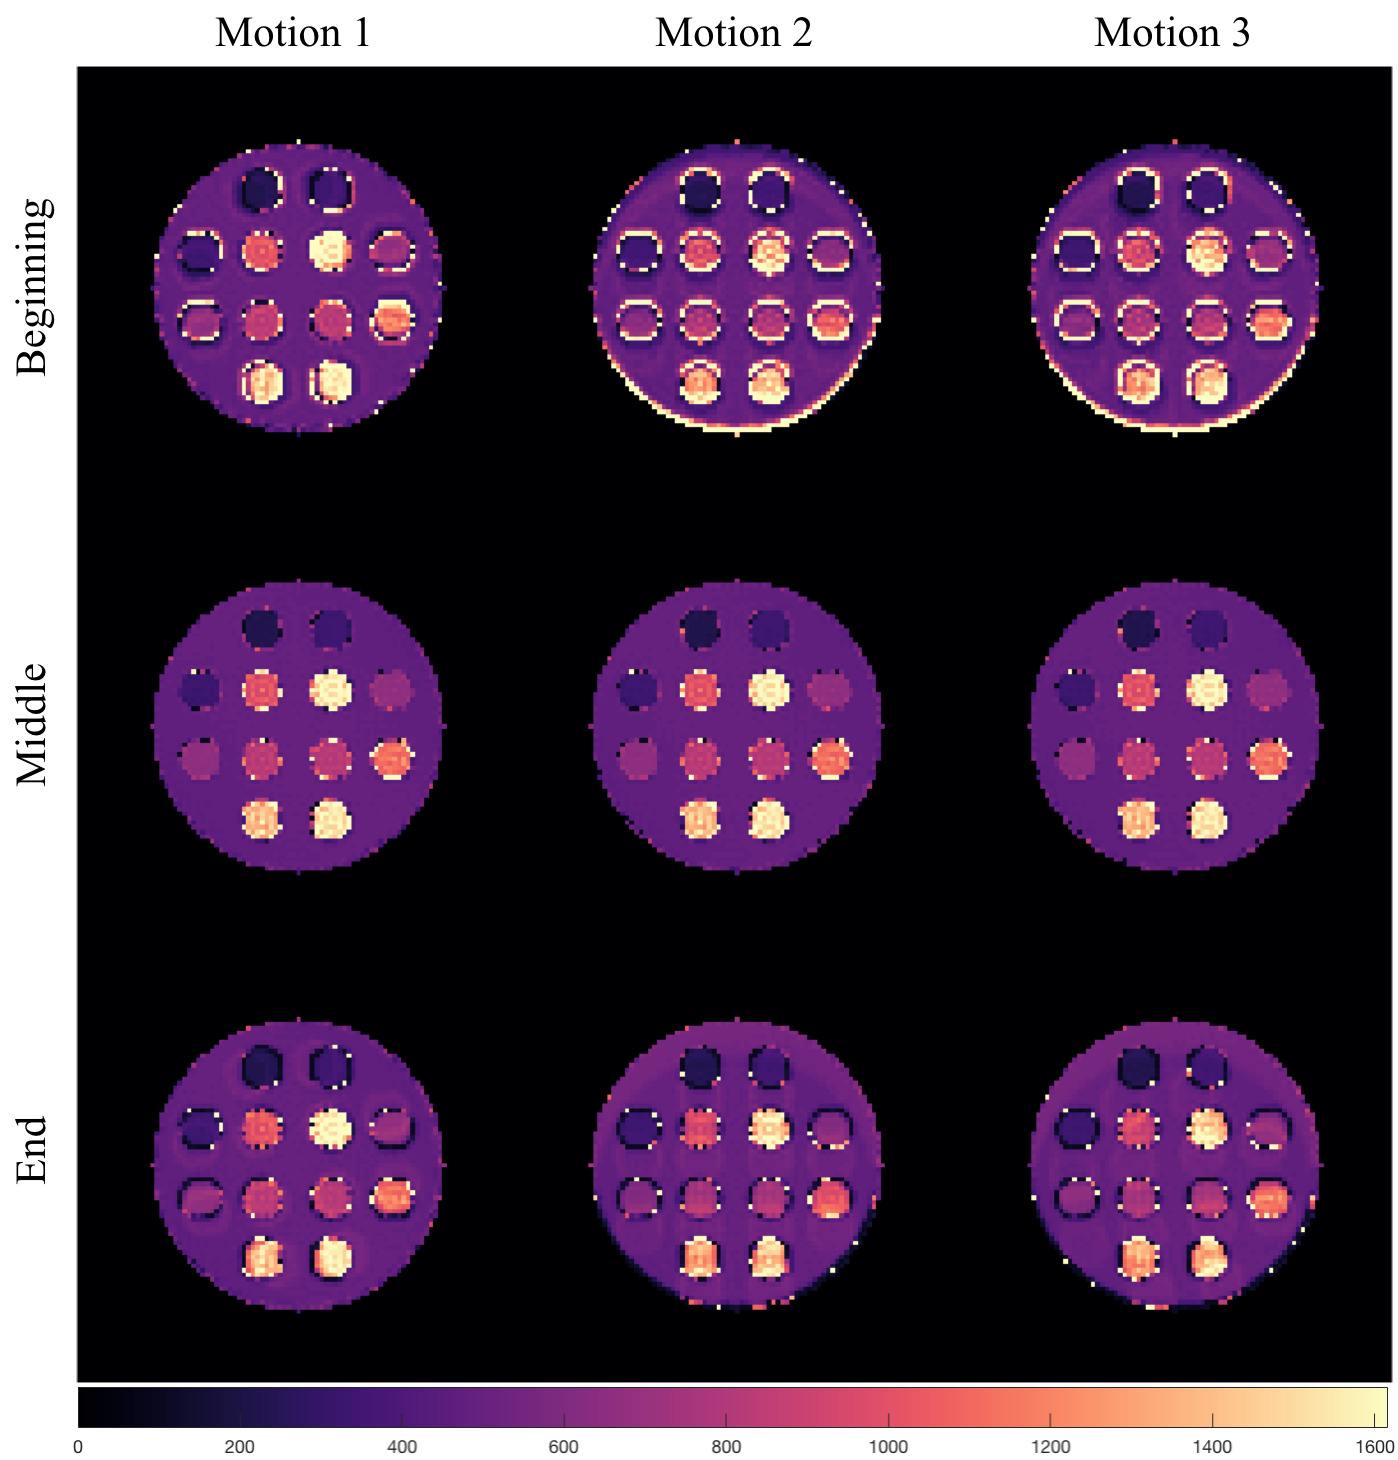
\includegraphics[width=0.85\textwidth]{images/mrf/T1mapsmotion}
%     \caption{Motion corrupted $T_1$ quantitative maps for all 9 types of motion traces. First column corresponds to the \textit{motion 1} trace (continuous rotation about the z-axis), the second column corresponds to the \textit{motion 2} trace (continuous translation along the y-axis) and the third column corresponds to the \textit{motion 3} trace (continuous rotation about the z-axis and continuous translation along the y-axis). Different lines correspond to a different onset of motion. }
%     \label{fig:T1mapsmotion}
% \end{figure}

% T2 maps motion
\begin{figure}[ht]
    \centering
    \begin{subfigure}[b]{.65\textwidth}
        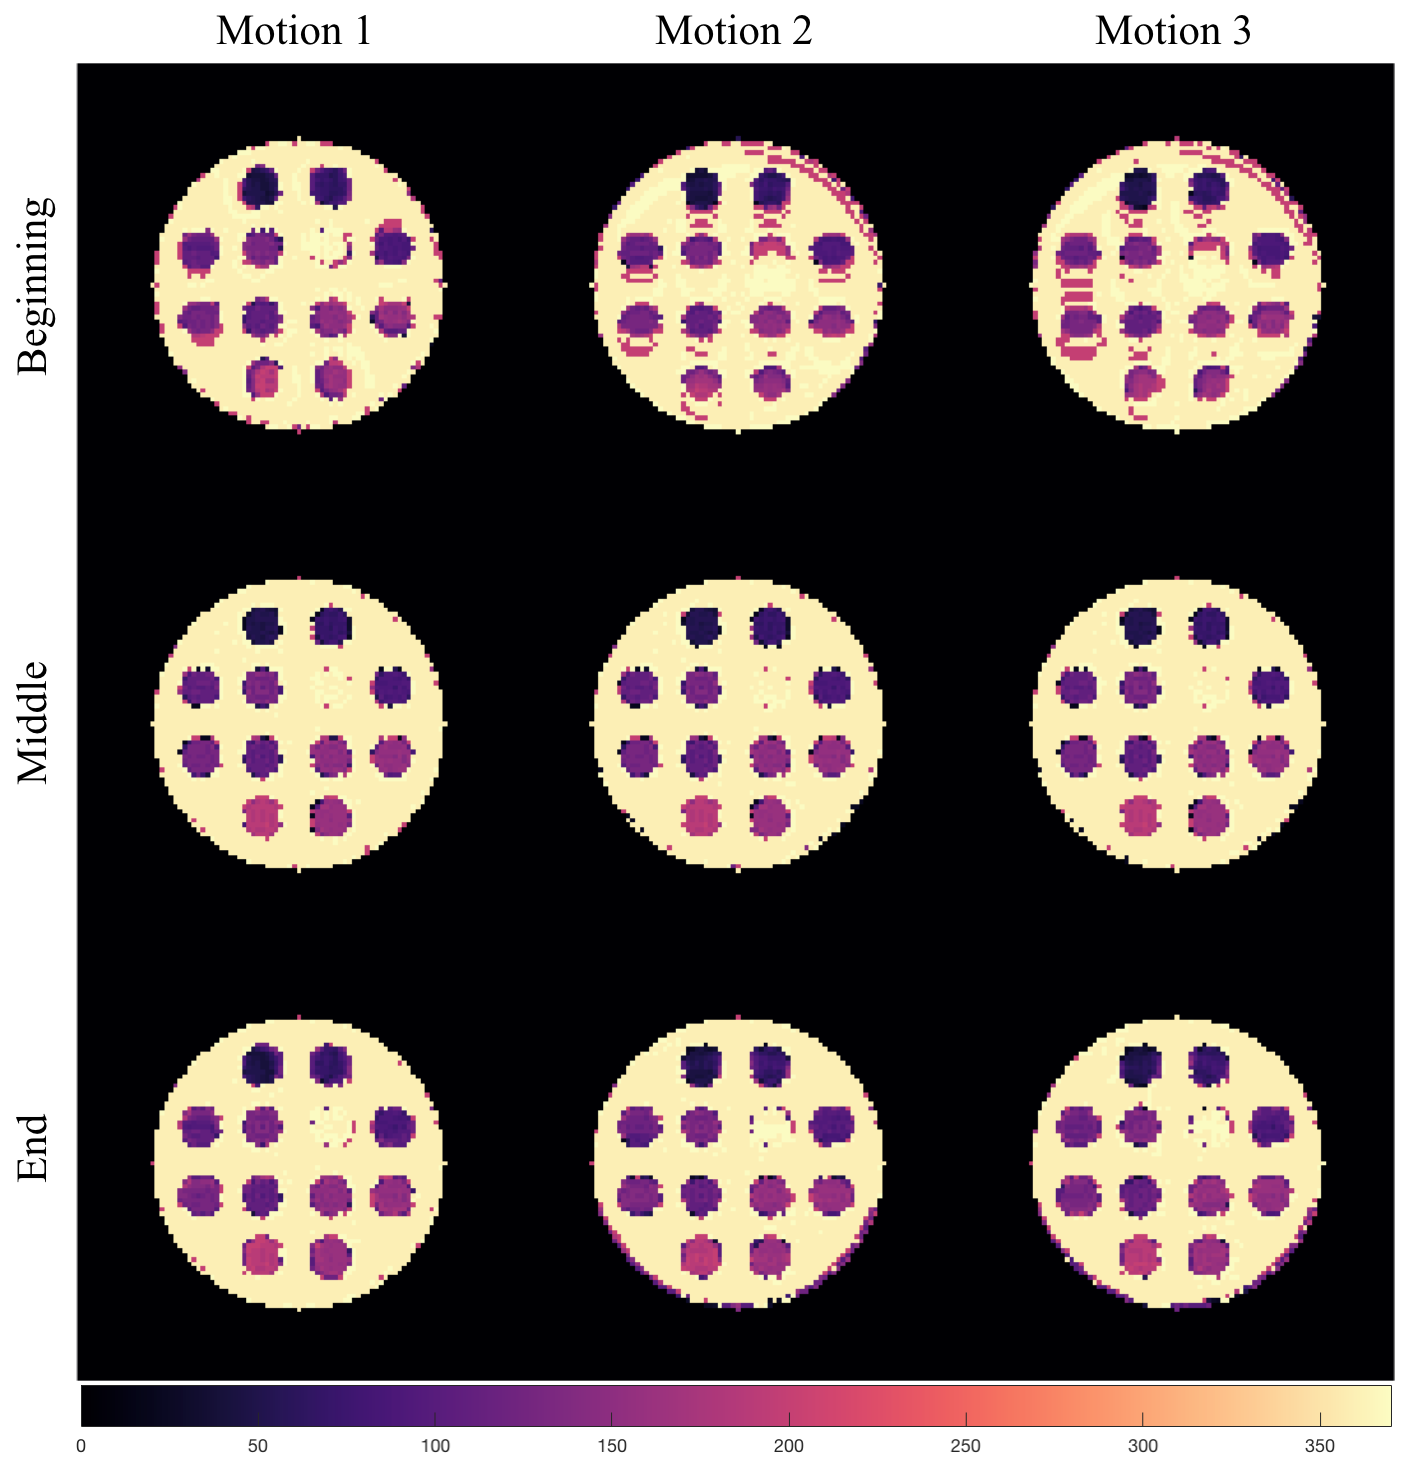
\includegraphics[width=\textwidth]{images/mrf/T2mapsmotion}
        \caption{Motion corrupted $T_2$ maps}
    \end{subfigure}
    
    \begin{subfigure}[b]{.65\textwidth}
        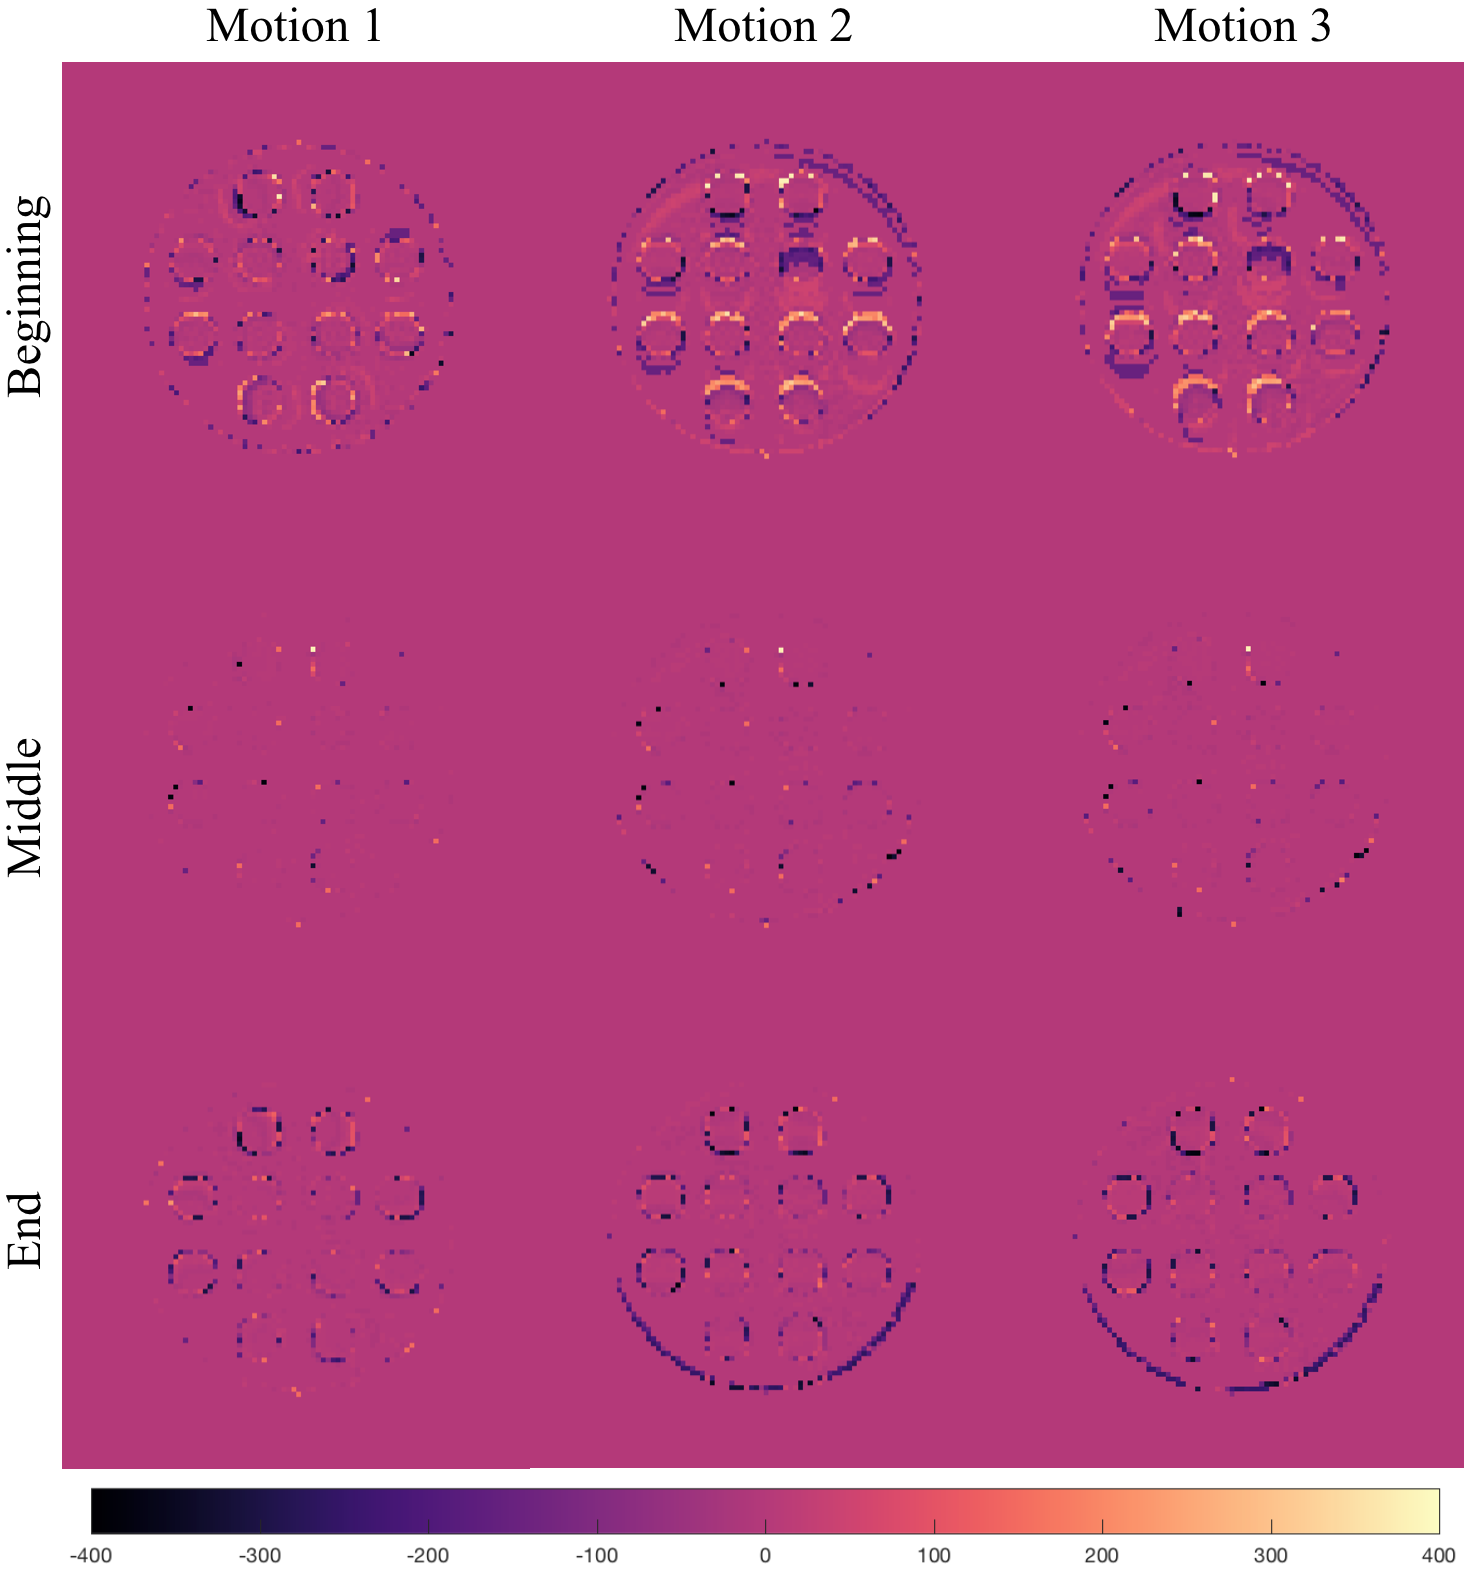
\includegraphics[width=\textwidth]{images/mrf/T2SimuMinusT2Real}
        \caption{Difference between $T_2^{motion \, \, corrupted}$ and $T_2^{motion \, \, free}$}
    \end{subfigure}
    
    \caption{Motion corrupted $T_2$ quantitative maps for all 9 types of motion traces. First column corresponds to the \textit{motion 1} trace (continuous rotation about the z-axis), the second column corresponds to the \textit{motion 2} trace (continuous translation along the y-axis) and the third column corresponds to the \textit{motion 3} trace (continuous rotation about the z-axis and continuous translation along the y-axis). Different lines correspond to a different onset of motion.}
    \label{fig:T2mapsmotion}
\end{figure}
% \begin{figure}[ht]
%     \centering
%     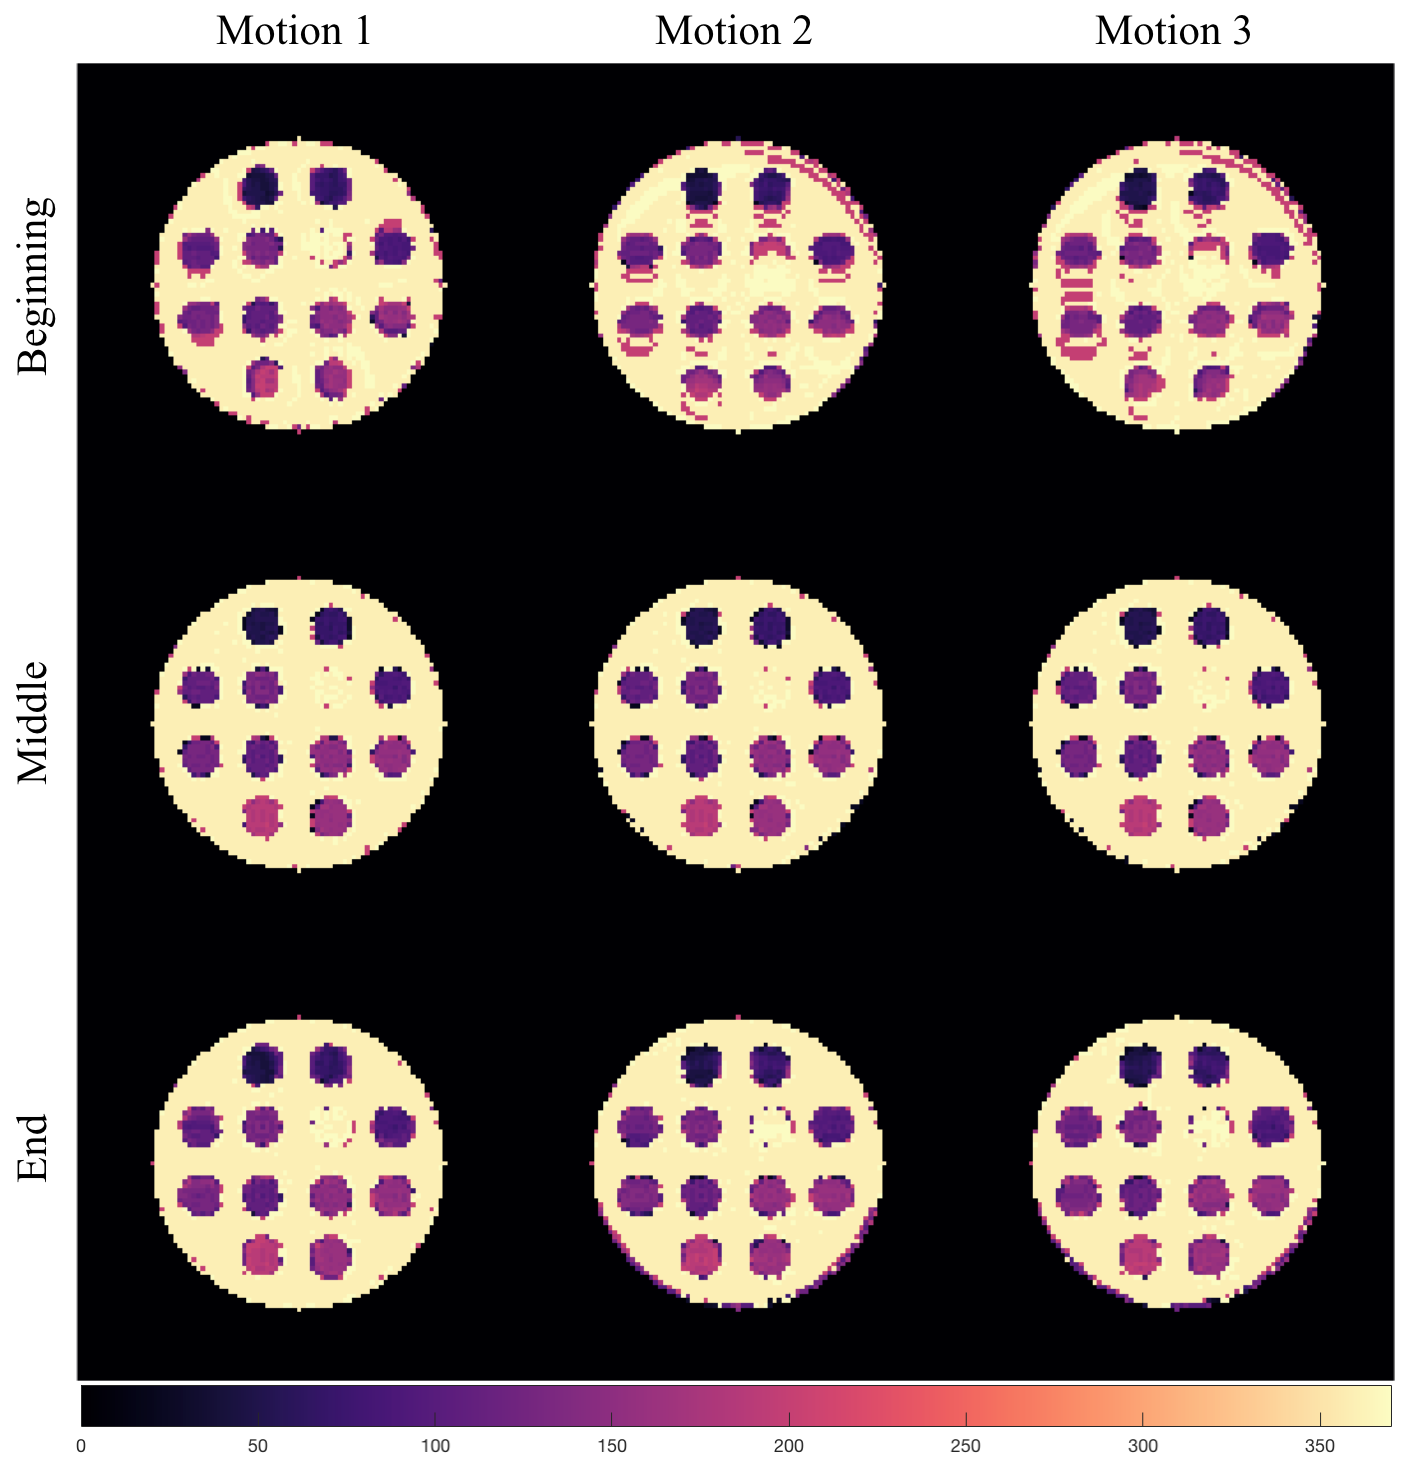
\includegraphics[width=0.85\textwidth]{images/mrf/T2mapsmotion}
%     \caption{Motion corrupted $T_2$ quantitative maps for all 9 types of motion traces. First column corresponds to the \textit{motion 1} trace (continuous rotation about the z-axis), the second column corresponds to the \textit{motion 2} trace (continuous translation along the y-axis) and the third column corresponds to the \textit{motion 3} trace (continuous rotation about the z-axis and continuous translation along the y-axis). Different lines correspond to a different onset of motion. }
%     \label{fig:T2mapsmotion}
% \end{figure}
% % % END images here:

% The other regions of interest are further from the centre and will all be affected by motion.
% More specifically, $T_2$ values are most affected when motion is happening at the beginning of the scan, regardless of the type of motion, and least affected when motion is happening in the middle or at the end of the scan.
% One potential reason for this is that the fingerprints are least discriminative in the middle of the scan for different $T_2$ values (see Figure~\ref{fig:mrfDictionaries} (b)).
% Similarly, $T_1$ values are also affected by motion happening at the beginning of the scan.
% In this case, small $T_1$ values (tubes 1 and 3) are always overestimated regardless of the type of motion, while higher $T_1$ values (tubes 5 and 12) are underestimated when translation is occurring.
% Moreover, motion occurring in the middle of the scan leads to overestimated high $T_1$ values (tubes 5 and 12), but does not affect lower $T_1$ values (tubes 1 and 3).

% \hfill

To further understand the impact of motion on the simulated maps, I decided to have a closer look at individual signals. 
Figure~\ref{fig:motion1ROIsignals} shows together the motion free signal (black dashed) and its dictionary match (green dashed), together with the motion corrupted signal (red) and its corresponding dictionary match (blue dashed), for continuous rotation with different onsets.
The plots show that the motion corrupted signal is matched to a different fingerprint than the motion free signal when the onset is at the beginning or at the end of the scan.
When motion is happening in the middle of the scan, the matching algorithm still finds the ground truth values.

% Motion 1 signals
\begin{figure}[ht]
    \centering
    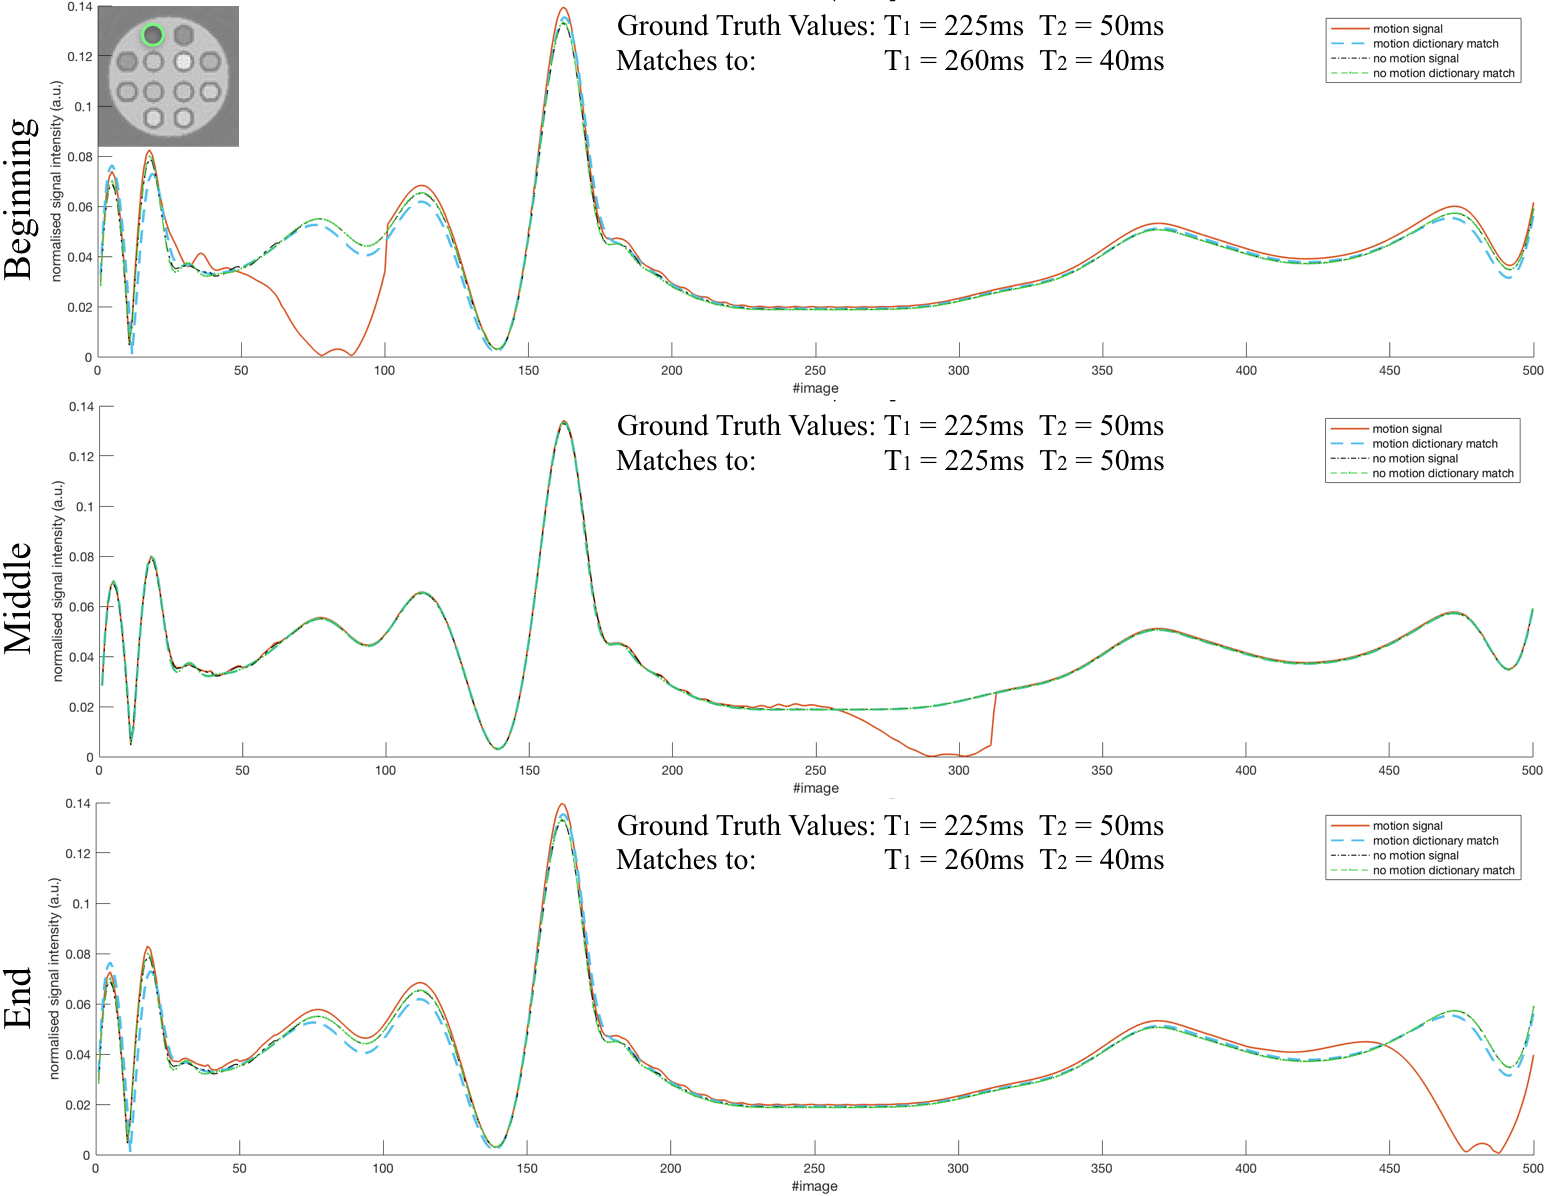
\includegraphics[width=0.95\textwidth]{images/mrf/motion1ROIsignals}
    \caption{Comparison between the motion free dictionary match and the motion corrupted dictionary match for different onsets of motion. Type of motion shown here is \textit{motion 1}.}
    \label{fig:motion1ROIsignals}
\end{figure}

\hfill

Figure~\ref{fig:motion2ROIsignals} shows a similar trend for the second type of motion.
However, in this plot a different voxel was chosen which corresponds to a higher $T_1$ value.
Here, all three types of onset affect the reconstructed values.
The least affected signal is, again, the one corresponding to motion happening in the middle of the scan, with the transverse relaxation time $T_2$ matched to the ground truth value of $160ms$.
As stated before, we speculate that the $T_2$ values are least affected here because the dictionary fingerprints are very similar to each other during the onset of motion (see  Figure~\ref{fig:problematicfingerprints}).

% Motion 2 signals
\begin{figure}[ht]
    \centering
    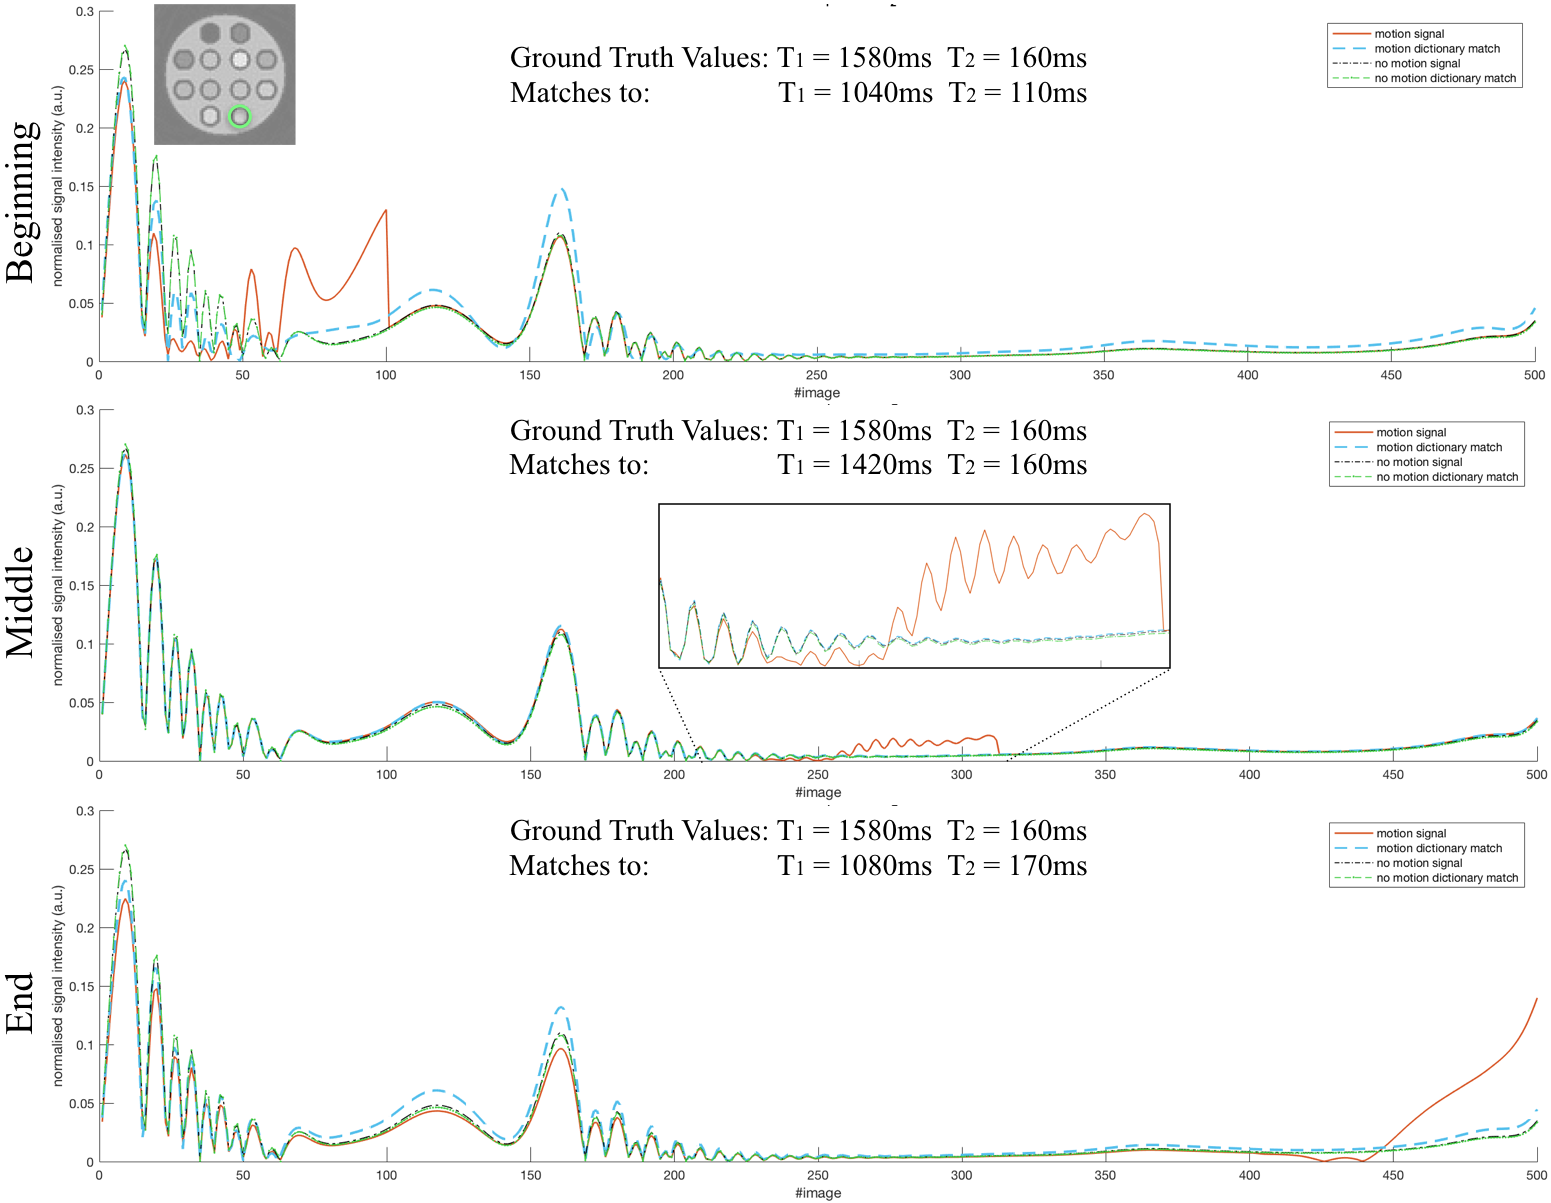
\includegraphics[width=0.95\textwidth]{images/mrf/motion2ROIsignals}
    \caption{Comparison between the motion free dictionary match and the motion corrupted dictionary match for different onsets of motion. Type of motion shown here is \textit{motion 2}.}
    \label{fig:motion2ROIsignals}
\end{figure}
